%% Cleaned Beamer file converted to Metropolis
\documentclass[english,aspectratio=169]{beamer}

% -------------------------------------------------
% Fonts and encoding
% -------------------------------------------------
\usepackage[T1]{fontenc}
\usepackage[latin9]{inputenc}
\usepackage{lmodern}
\renewcommand{\sfdefault}{lmss}
\renewcommand{\ttdefault}{lmtt}

% -------------------------------------------------
% Language and layout
% -------------------------------------------------
\usepackage{babel}
\setlength{\parskip}{\medskipamount}
\setlength{\parindent}{0pt}

% -------------------------------------------------
% Math, graphics, listings
% -------------------------------------------------
\usepackage{amssymb}
\usepackage{amsmath}
\usepackage{graphicx}
\usepackage{color}
\usepackage{tikz}
\usepackage{listings}
\renewcommand{\lstlistingname}{Listing}
\usepackage{media9}   % modern package for embedding video

% -------------------------------------------------
% Theme: Metropolis
% -------------------------------------------------
\usetheme{metropolis}
\metroset{progressbar=frametitle,sectionpage=progressbar}

% -------------------------------------------------
% UCT Brand Colors
% -------------------------------------------------
\definecolor{UCTBlue}{HTML}{009ADA}
\definecolor{UCTDarkBlue}{HTML}{00243A}

\setbeamercolor{palette primary}{bg=UCTDarkBlue, fg=white}
\setbeamercolor{frametitle}{bg=UCTDarkBlue, fg=white}
\setbeamercolor{progress bar}{fg=UCTBlue}
\setbeamercolor{title separator}{fg=UCTBlue}
\setbeamercolor{alerted text}{fg=UCTBlue}

% -------------------------------------------------
% Custom UCT title slide
% -------------------------------------------------
\setbeamertemplate{title page}{%
  \begin{tikzpicture}[remember picture,overlay]
    % Background
    \fill[UCTBlue] (current page.south west) rectangle (current page.north east);
    % Logo
    \node[anchor=north, xshift=-4cm, yshift=-1.2cm] at (current page.north)
      {\includegraphics[height=1cm]{uct_logo_horizontal_white}};
    \node[anchor=north, xshift=4cm, yshift=0cm] at (current page.north)
      {
\includegraphics[height=3cm]{samos-logo-transparent}};      
  \end{tikzpicture}
  \vspace*{3.2cm}
  \begin{center}
    {\usebeamercolor[fg]{title}\usebeamerfont{title}\textcolor{white}{\inserttitle}}\\[0.6em]
    {\usebeamerfont{subtitle}\textcolor{white}{\insertsubtitle}}\\[1.2em]
    {\usebeamerfont{author}\textcolor{white}{\insertauthor}}\\[0.3em]
    {\usebeamerfont{institute}\textcolor{white}{\insertinstitute}}\\[0.8em]
    {\usebeamerfont{date}\textcolor{white}{\insertdate}}
  \end{center}
}

% -------------------------------------------------
% Footer logo for content slides
% -------------------------------------------------
\usepackage{tikzpagenodes}
\addtobeamertemplate{footline}{}{%
  \begin{tikzpicture}[remember picture,overlay]
    \node[anchor=south east, xshift=-1cm, yshift=0cm]
      at (current page.south east)
      {\includegraphics[height=0.5cm]{uct_logo_horizontal_blue}};
    \node[anchor=south west, xshift=0cm, yshift=-0.2cm]
      at (current page.south west)
      {
\includegraphics[height=0.7cm]{samos-logo-transparent.png}};  
  \end{tikzpicture}%
}

% -------------------------------------------------
% LyX-specific definitions (kept minimal)
% -------------------------------------------------
\makeatletter

\newcommand\makebeamertitle{\frame{\maketitle}}

\AtBeginDocument{%
  \let\origtableofcontents=\tableofcontents
  \def\tableofcontents{\@ifnextchar[{\origtableofcontents}{\gobbletableofcontents}}
  \def\gobbletableofcontents#1{\origtableofcontents}
}

\newenvironment{lyxcode}
  {\begin{list}{}{
     \setlength{\rightmargin}{\leftmargin}
     \setlength{\listparindent}{0pt}
     \setlength{\itemsep}{0pt}
     \setlength{\parsep}{0pt}
     \raggedright\normalfont\ttfamily
   }\item[]}
  {\end{list}}

\makeatother

% -------------------------------------------------
% Document
% -------------------------------------------------
\begin{document}

    \title[US2.4-bgc]{Introduction to biogeochemical modelling}
    \author{Marcello Vichi}
    \institute[UCT]{Department of Oceanography\\marcello.vichi@uct.ac.za}
    \date{AOS-SAMOS}
    \maketitle

\begin{frame}{Outline}
    \tableofcontents{}
\end{frame}

%------------------------------------------------
\section{A brief history of ecosystem/biogeochemical modelling}
%------------------------------------------------
\begin{frame}{Biogeochemical modelling}
\begin{itemize}
\item Integration of physics, chemistry, biology
\item The governing equations of chemical-biological systems cannot be derived from conservation laws such as Newton’s Mechanics or Geophysical Fluid Dynamics.
\item The equations of biology must be derived empirically (heuristically) and require several assumptions on the choice of state variables and dynamics (parameterizations)
\item But what are the stocks and flows?
\end{itemize}

\medskip
\textbf{Generic mass balance:}
\[
\frac{dC}{dt} = \text{Sources} - \text{Sinks}
\]
\end{frame}

%------------------------------------------------
\begin{frame}{The trophic dynamic viewpoint}
\begin{columns}
\column{0.5\linewidth}
\begin{figure}
    \centering
    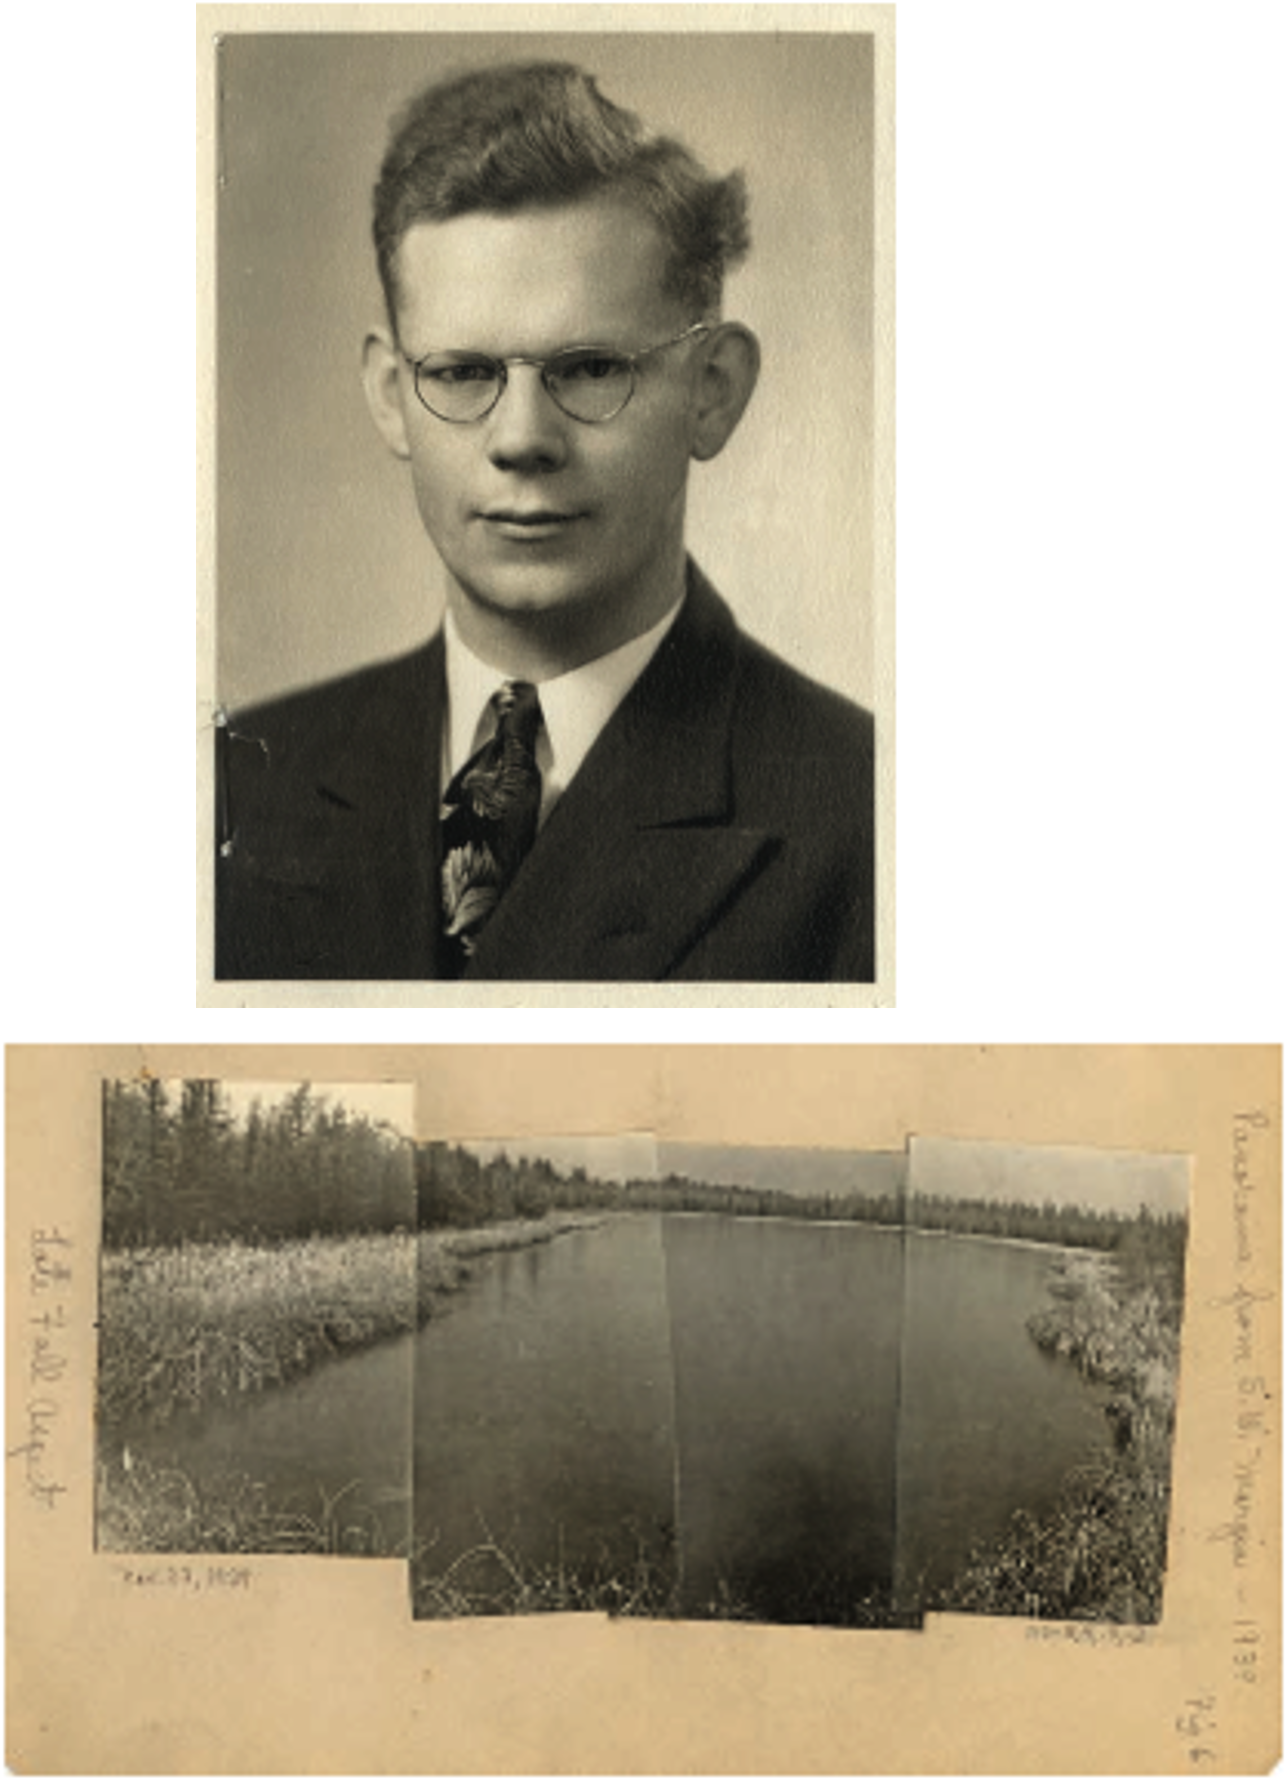
\includegraphics[width=0.75\linewidth]{figures/lindeman.png}
\end{figure}
\column{0.6\linewidth}
\begin{itemize}
\item Raymond L. Lindeman (1915--1942). Lindeman, R. L. 1942.The trophic-dynamic aspect of ecology. Ecology 23:399-418.
\item For the first time Lindeman formalized a description of Cedar Bog Lake in Minnesota with a Food Cycle diagram, a “wiring diagram”.
\item Breakthrough two was the quantification of stocks and rates that layered on top of that diagram. (Sterner, ASLO Bullettin, 12, 2012)
\end{itemize}
\[
\frac{dB_i}{dt} = \sum F_{in} - \sum F_{out}
\]
\end{columns}
\end{frame}




%------------------------------------------------
\begin{frame}{System state variables}
\begin{columns}
\column{0.5\linewidth}
Representation of the main trophic levels and groups that were considered state variables of the system.

Lindeman went beyond the simple conceptual drawing as he computed the stocks and flows through careful accounting of biomass transfer in terms of $gC\, m^{-2}$.
\column{0.5\linewidth}
\begin{figure}
    \centering
    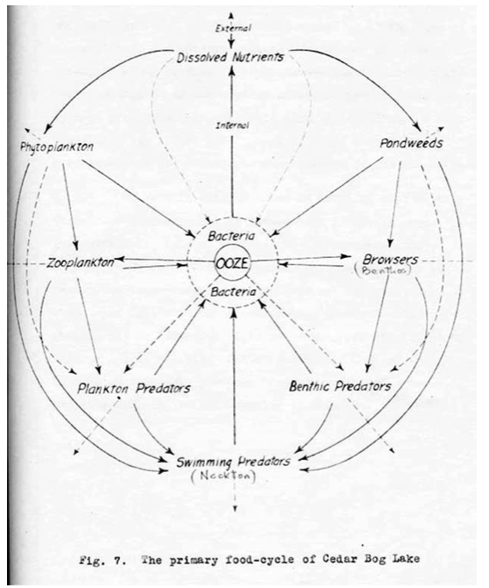
\includegraphics[width=1\linewidth]{figures/lindeman-diagram.png}
\end{figure}
\end{columns}
\end{frame}

%------------------------------------------------
\begin{frame}{Ocean energy as a shaping factor}
\small{
\begin{itemize}
\item The environment remained hidden until the 70s. Ramon Margalef's (1978) pioneering work stated: \textit{the best predictor of primary production and of dominant life-forms in phytoplankton is the available external energy, on which advection and turbulence depend. \textbf{This factor overrules more detailed models using light and nutrients} as most relevant parameters, and based on laboratory experiments.}
$P \sim f(E_{\text{turbulence}}, E_{\text{advection}})$
\item The spatial structure of data must be carefully maintained (Margalef, 1985)
\end{itemize}
}
\vspace{-0.5cm}
\begin{figure}
    \centering
    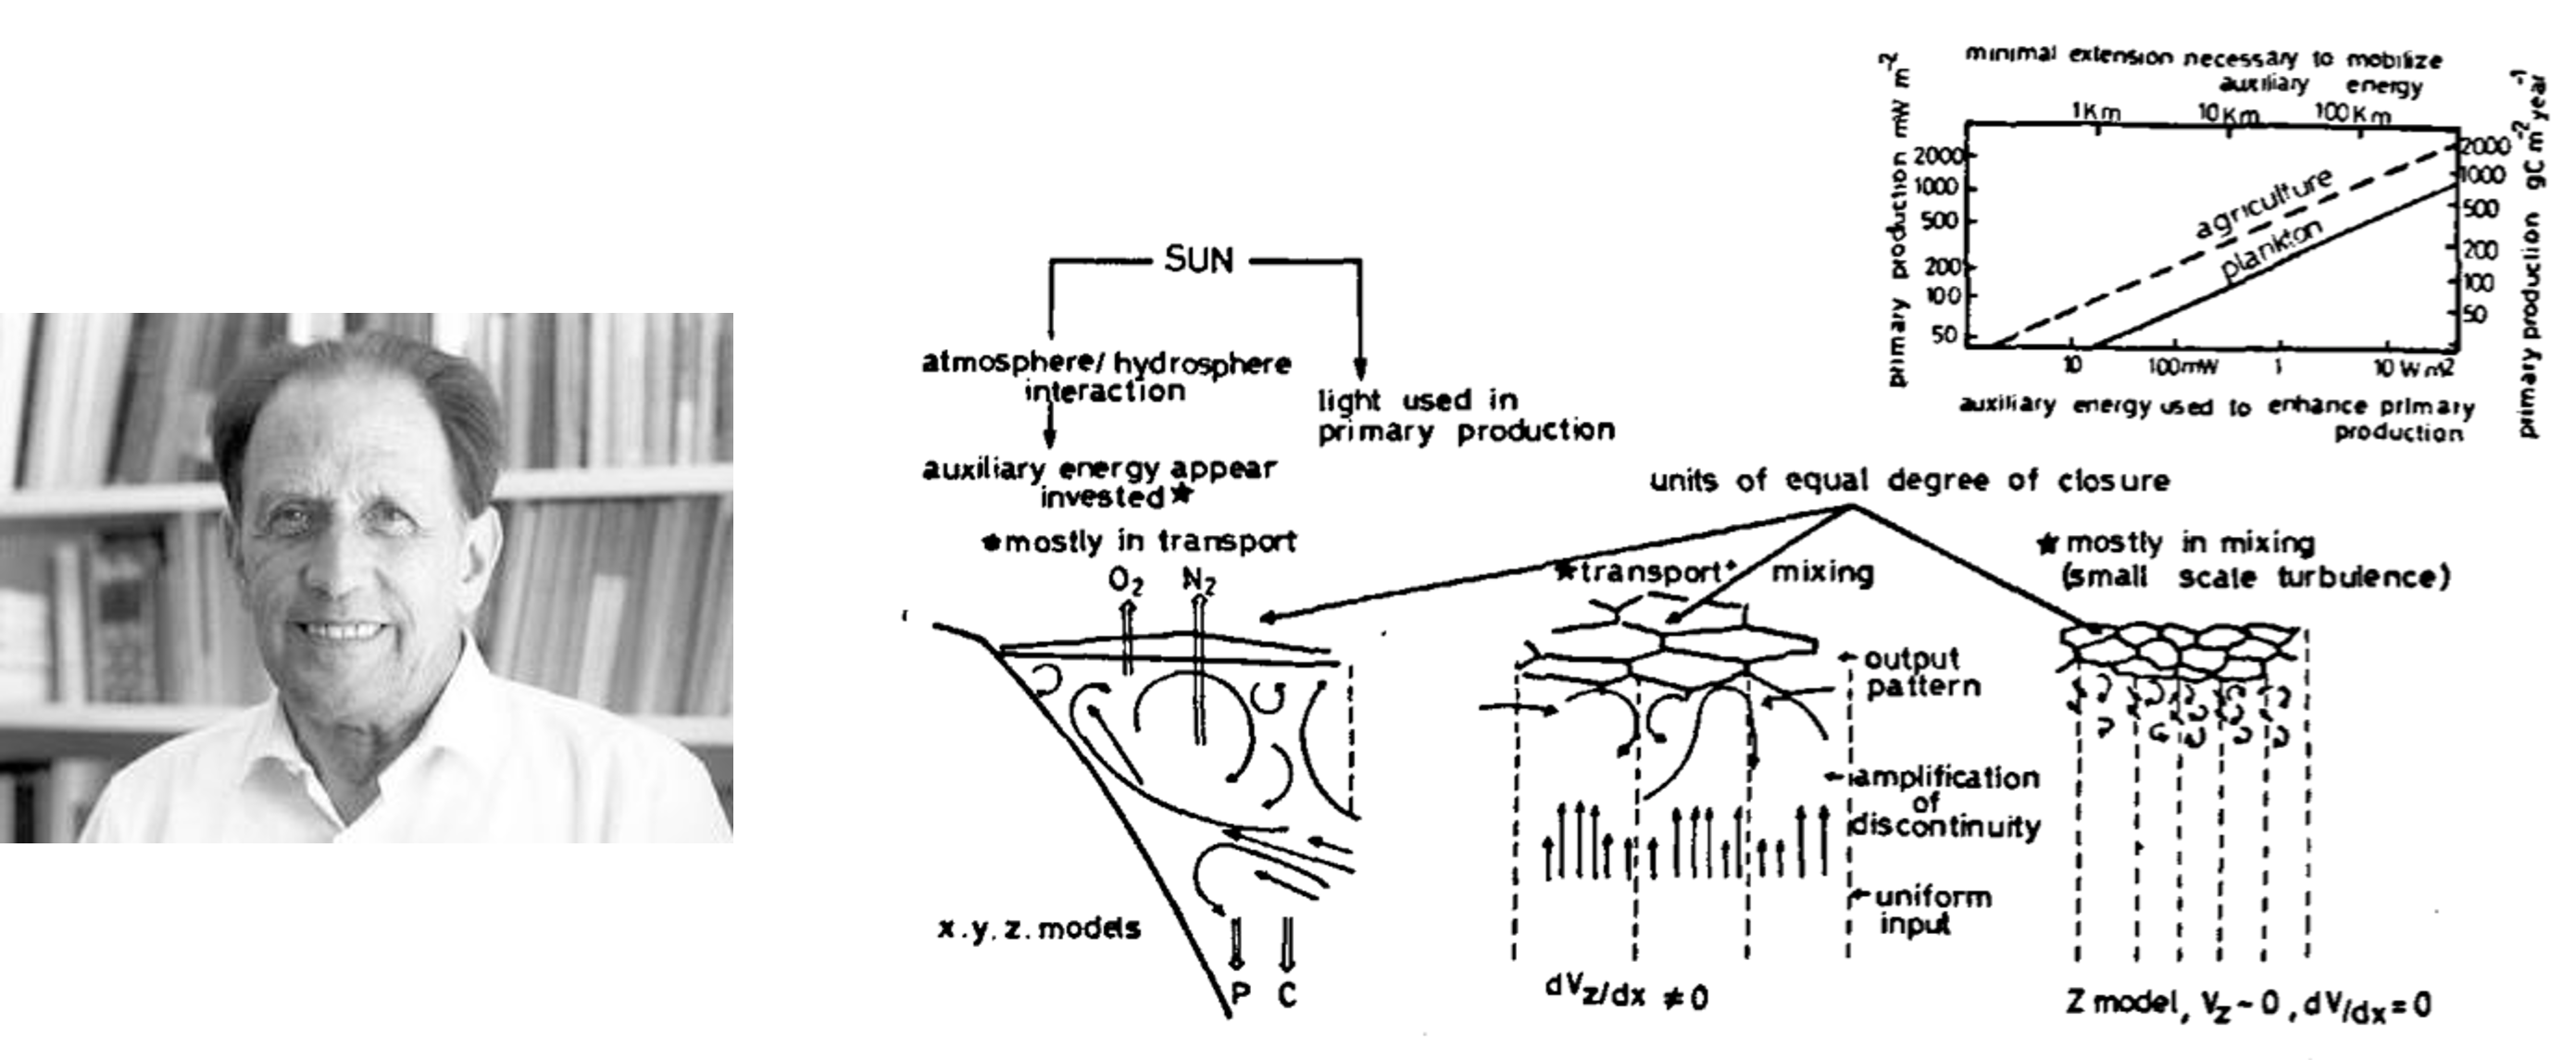
\includegraphics[width=0.7\linewidth]{figures/margalef.png}
\end{figure}
\end{frame}

%------------------------------------------------
\begin{frame}{The microbiome}
\begin{figure}
    \centering
    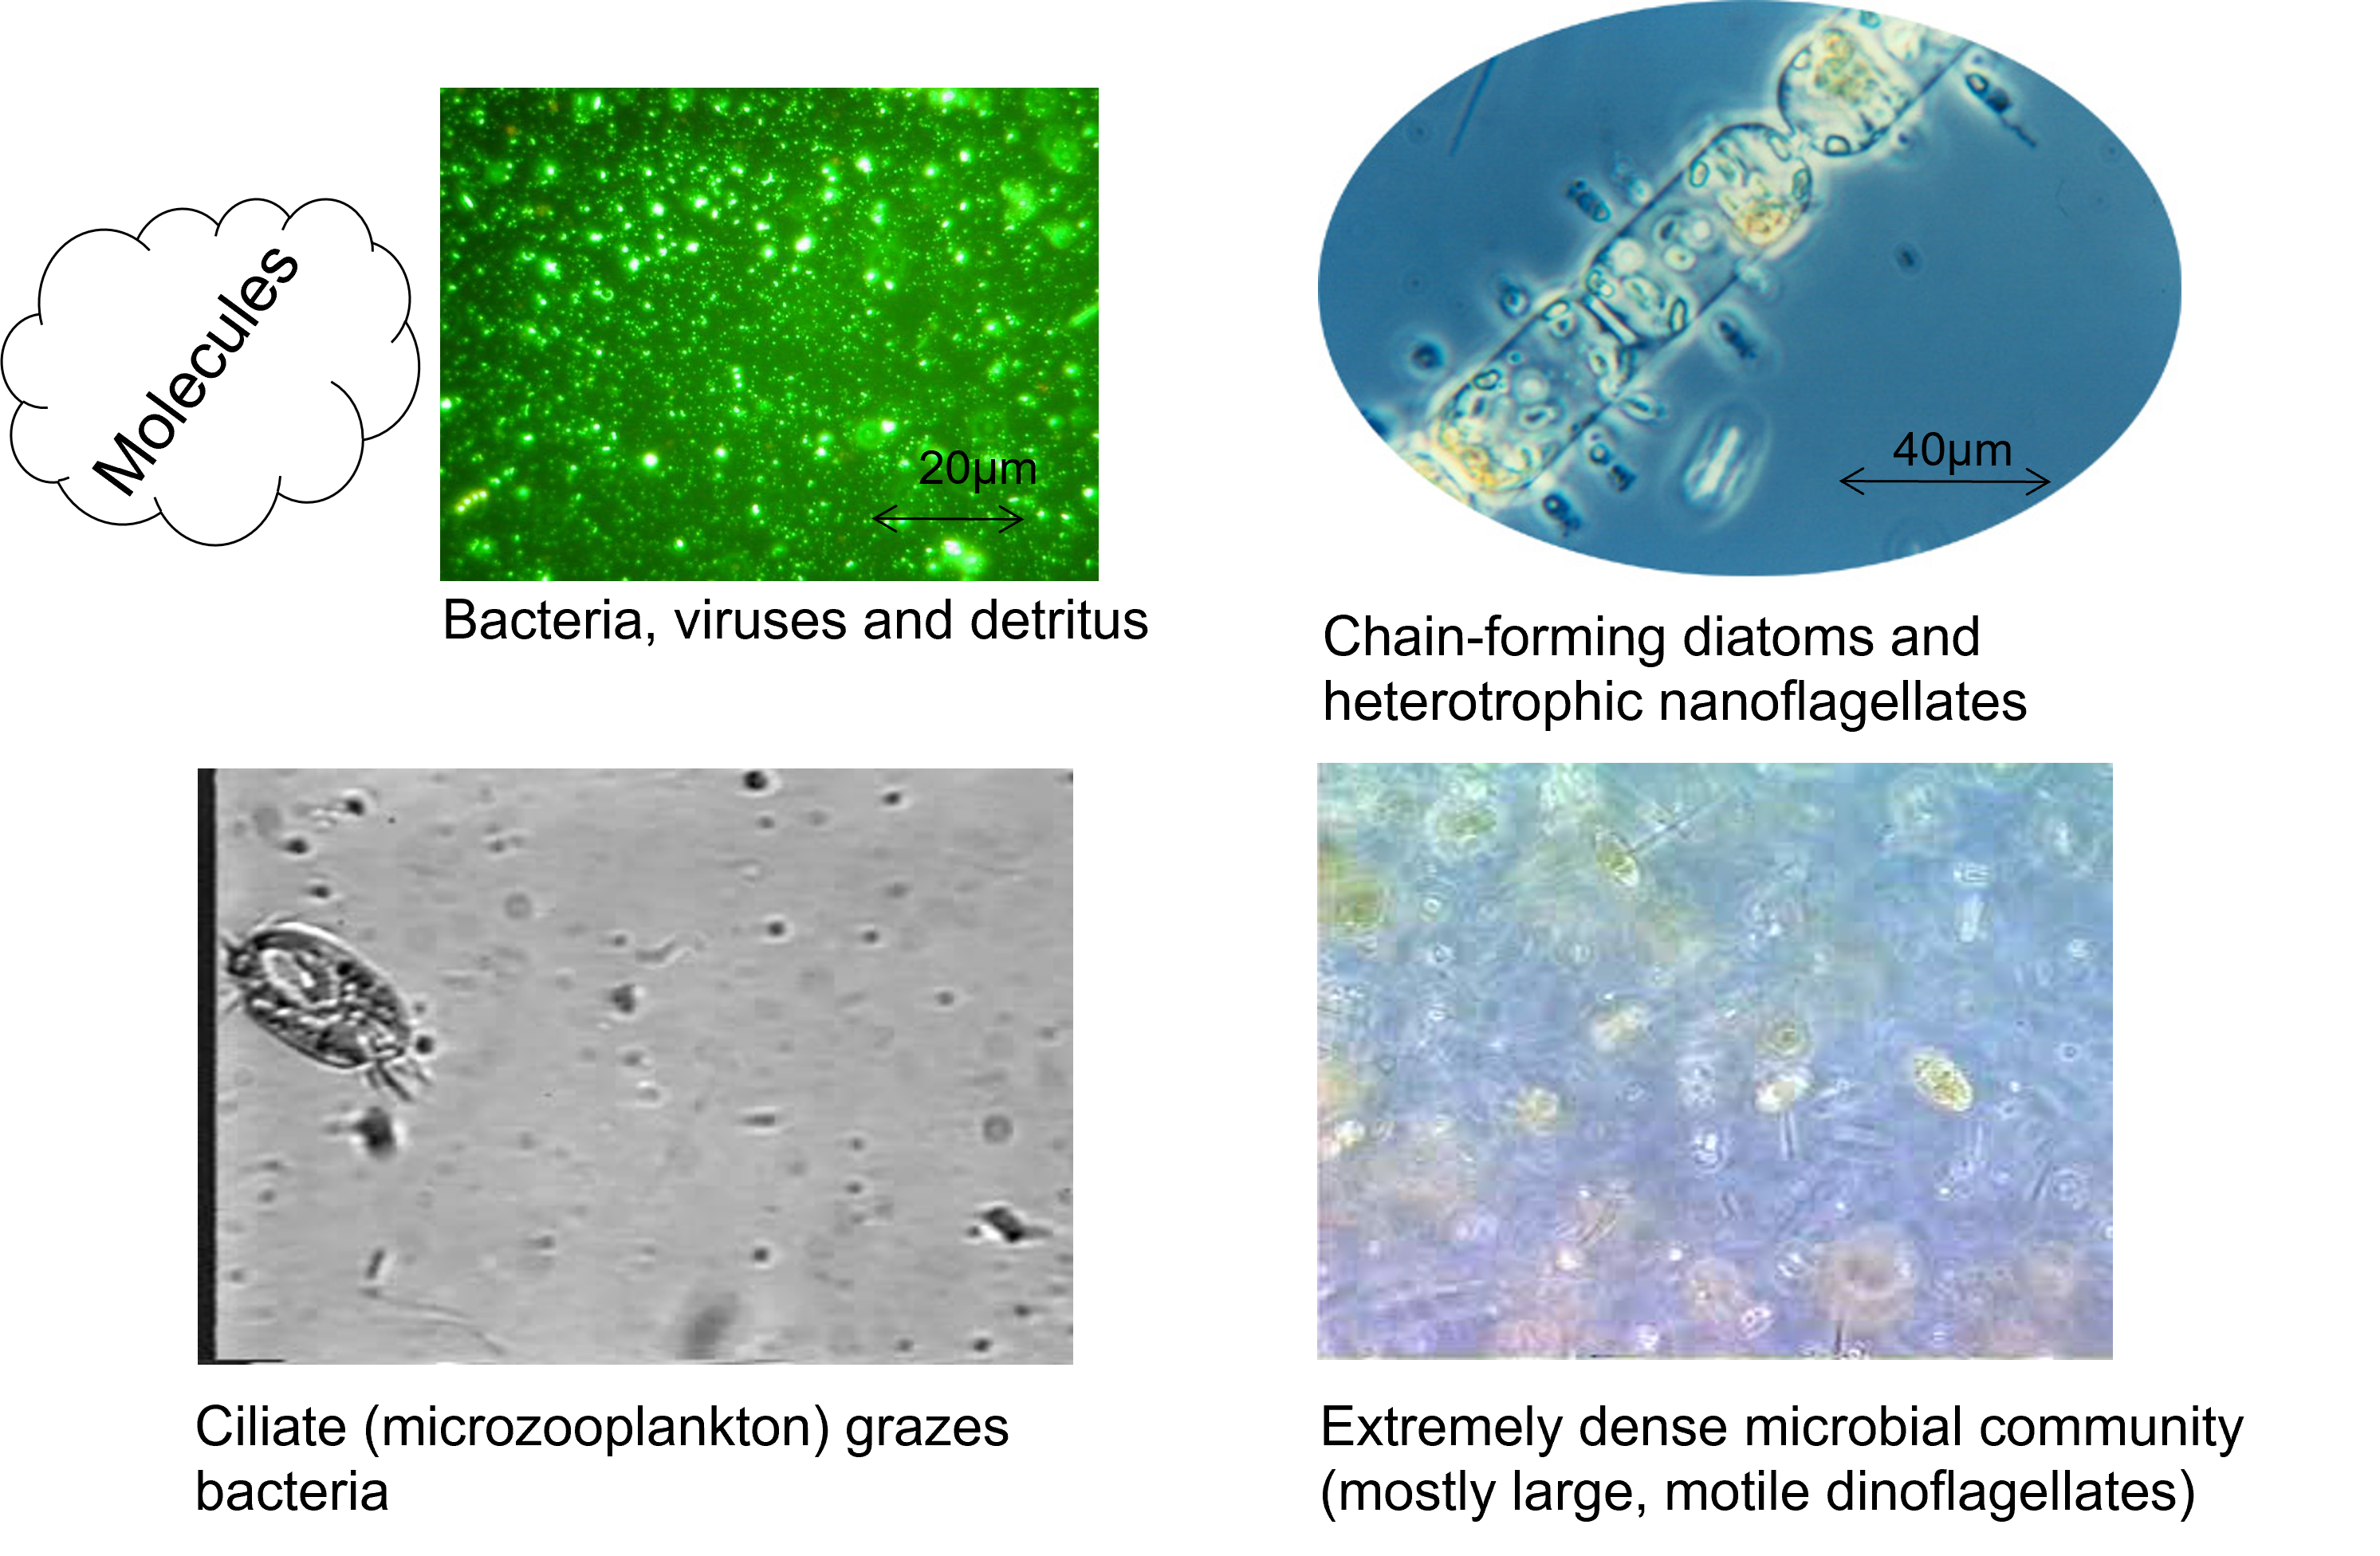
\includegraphics[width=0.7\linewidth]{figures/microbiome.png}
\end{figure}
\end{frame}

%------------------------------------------------
\begin{frame}{Biological Time-space scales}
\begin{figure}
    \centering
    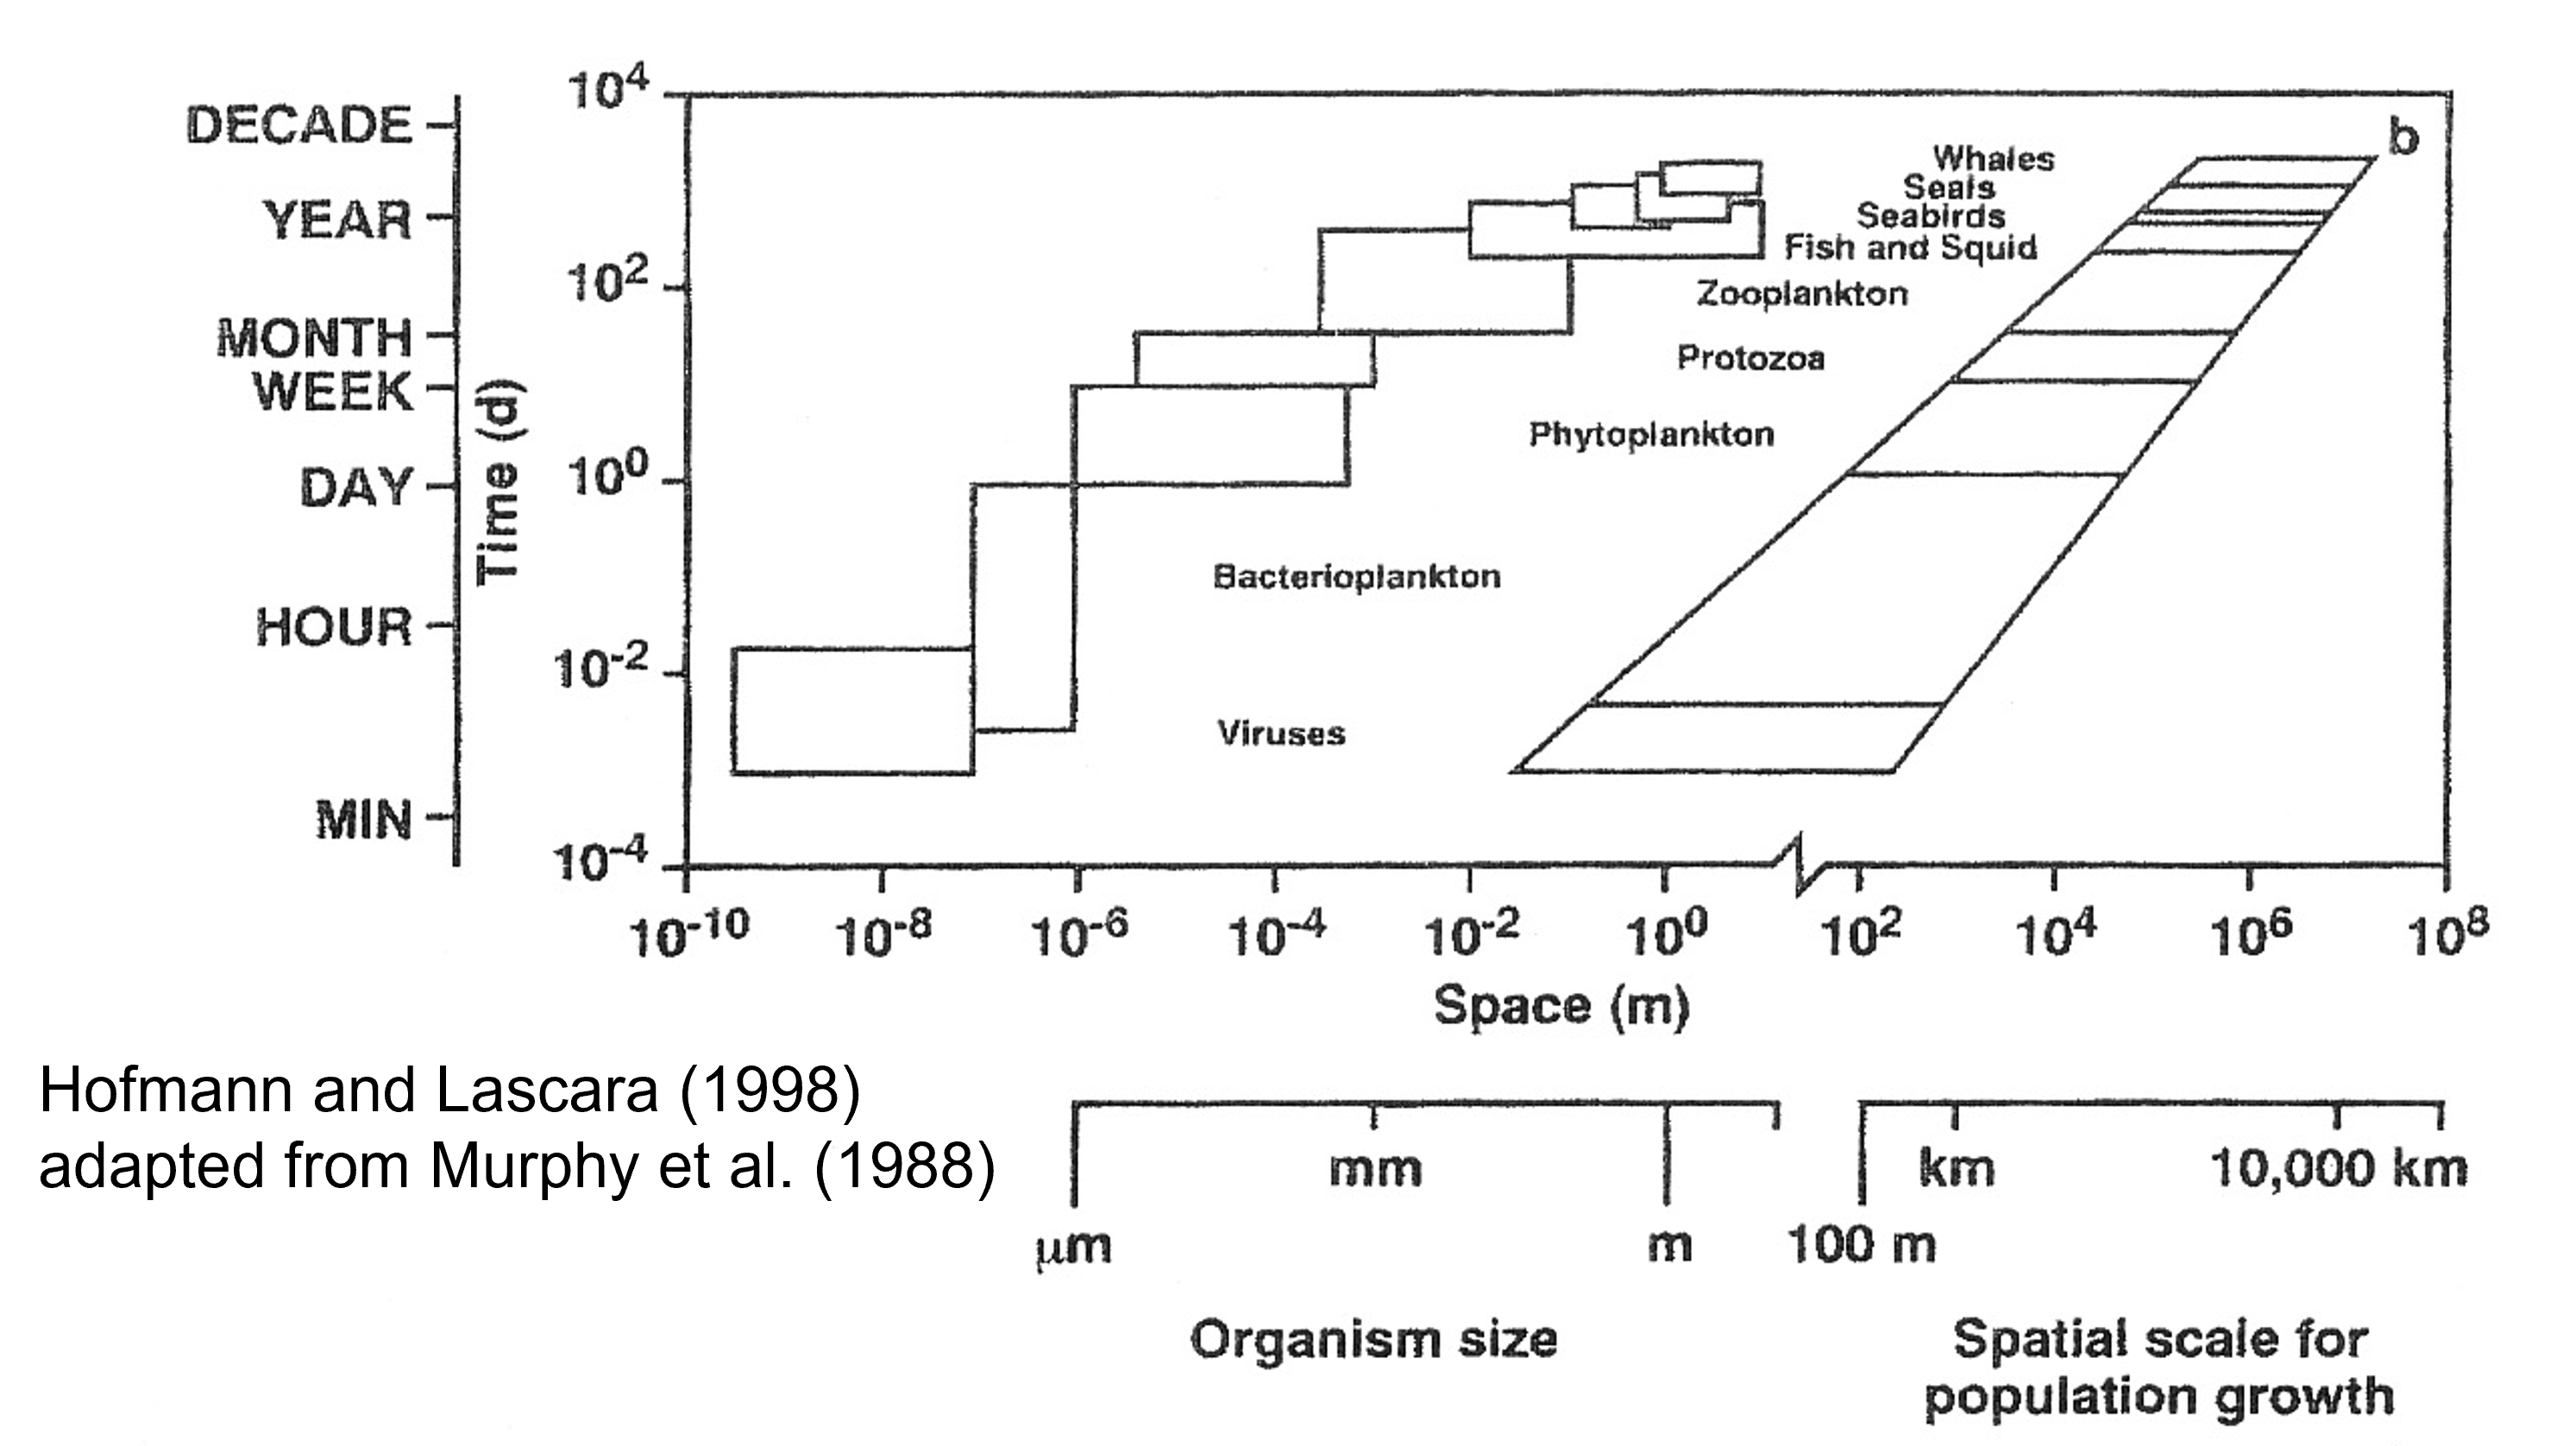
\includegraphics[width=0.9\linewidth]{figures/microbiome_scales.png}
\end{figure}
\end{frame}

%------------------------------------------------
\begin{frame}{Early plankton models}
\begin{itemize}
\item The first mathematical models for planktonic ecosystems were developed in the late 1940s (Riley, 1946, 1947; Georges Bank)
\item They included time-dependent processes for phytoplankton and zooplankton as dynamics of populations with equal individuals (extension of the prey-predator population model of Volterra-Lotka, more on this later). Founding concept of bulk biomass models.
\item The environment was not explicitly modelled.
\end{itemize}
\end{frame}

%------------------------------------------------
\begin{frame}{Types of models}
\begin{itemize}
\item \textbf{Individual-based (IBM)} The properties of each individual are treated separately (behavioural models with ontogenetic processes) and can also include genetic variations (phylogenetic processes)
\item \textbf{Population models} The properties are averaged over the individuals (discarding internal variability) and the state variable is normally the number of individuals in each population considered (size-classes, cohorts)
\item \textbf{Biomass-based models} Similar to population models but uses mass concentration  units as state variables, assuming that this mass is a measurable quantity and characterize the functioning of the population (e.g. Nitrogen-based models). Generally used for lower trophic levels (where the increase in population number equals the growth in bulk biomass)
\item \textbf{Combinations} End-to-End models
\end{itemize}
\end{frame}

%------------------------------------------------
\begin{frame}{Biomass-based models}
\begin{itemize}
    \item Prototype: chemical reaction $\text{Reaction form: } A + B \rightarrow C$
    \item Simple models: Nutrient-Phytoplankton with one constituent
    \item Simple models of shallow systems: NPZD with one constituent
    \item Fasham-like models with one constituent
    \item Comprehensive models of marine biogeochemistry (ERSEM-like) with multiple constituents. Plankton Functional Types or Green Models
\end{itemize}

\end{frame}

%------------------------------------------------
\begin{frame}{The first correlation between environment and plankton growth: Riley model}
\begin{columns}
\column{0.4\linewidth}
The Riley model (1946, 1947) was the first to calculate statistical correlations between environmental variables and phytoplankton biomass (in concentration of plant pigments $m^{-2}$). 
\[
\text{Biomass} \propto \text{light} \times \text{nutrients}
\]
\column{0.7\linewidth}
\begin{figure}
    \centering
    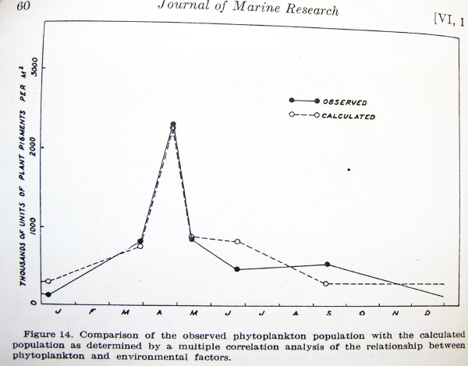
\includegraphics[width=0.9\linewidth]{figures/riley.png}
\end{figure}
\end{columns}
\end{frame}

%------------------------------------------------
\begin{frame}{The Fasham's legacy}
\begin{columns}
\column{0.5\linewidth}
\begin{figure}
    \centering
    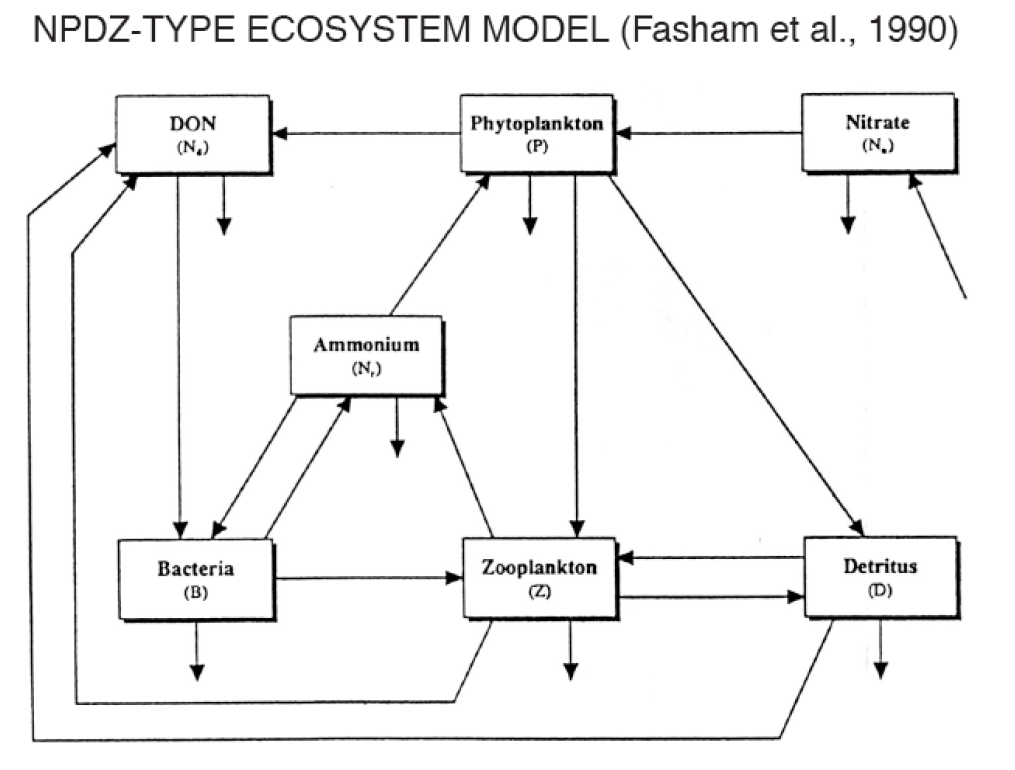
\includegraphics[width=1\linewidth]{figures/fasham90.png}
\end{figure}
\column{0.5\linewidth}
\begin{itemize}
\small
    \item After Jamart et al. (1977), who simulated the vertical profile of chlorophyll in idealised conditions, Fasham et al. (1990) were the first to explicitly include coupled physical and biogeochemical processes in a realistic context to simulate the North Atlantic sub-polar bloom (\url{https://marine.copernicus.eu/news/north-atlantic-ocean-bloom-and-why-it-matters}). 
    \item The model had multiple state variables (compartments), one currency (N, constituent), and set the stage for most of the future ocean biogeochemistry models (OBM).
\end{itemize}
\end{columns}
\end{frame}

%------------------------------------------------
\begin{frame}{The ERSEM legacy}
\begin{columns}
\column{0.3\linewidth}
The European Regional Seas Ecosystem Model was the first of its kind to combine lower and higher trophic levels, including benthic-pelagic coupling. It was implemented on a very coarse grid in the North Sea, but since then it evolved in two different branches, the \href{https://pml.ac.uk/projects/ersem-european-regional-seas-ecosystem-model/}{PML ERSEM} and the \href{https://www.bfm-community.eu/}{Biogeochemical Flux Model}.
\column{0.7\linewidth}
\begin{figure}
    \centering
    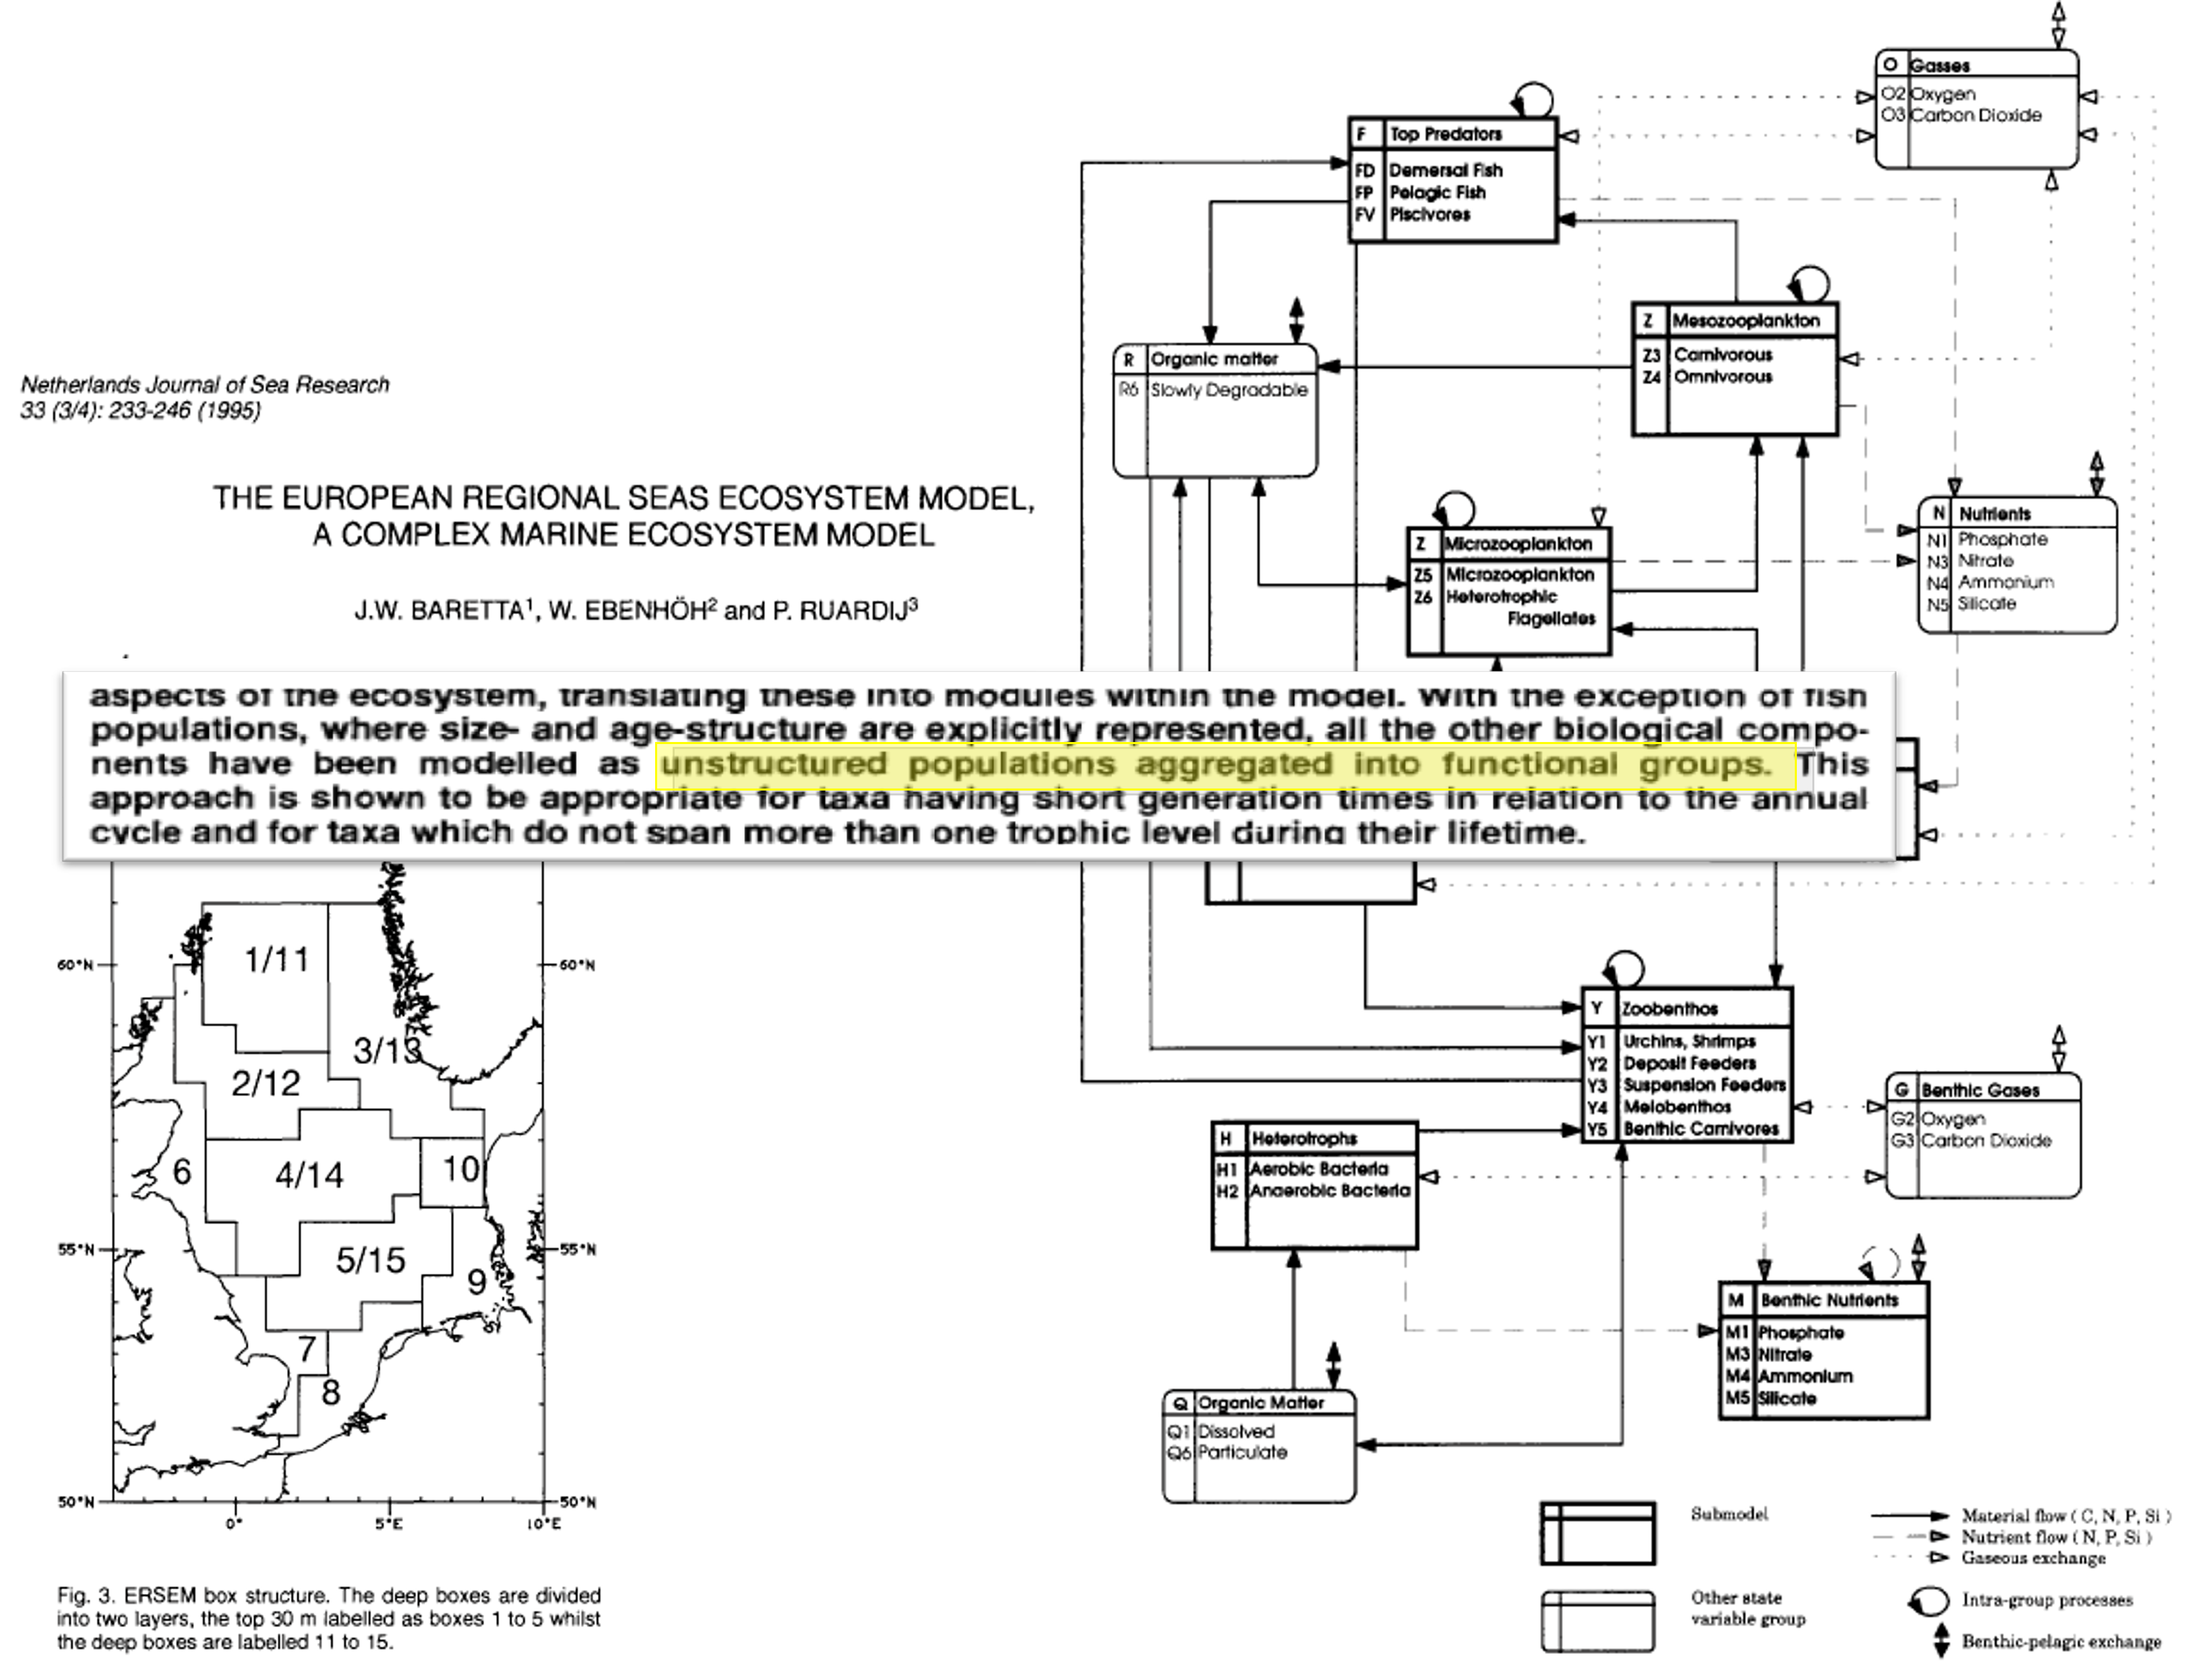
\includegraphics[width=1\linewidth]{figures/ERSEM.png}
\end{figure}
\end{columns}
\end{frame}
%------------------------------------------------
\begin{frame}{Model complexity}
\begin{figure}
    \centering
    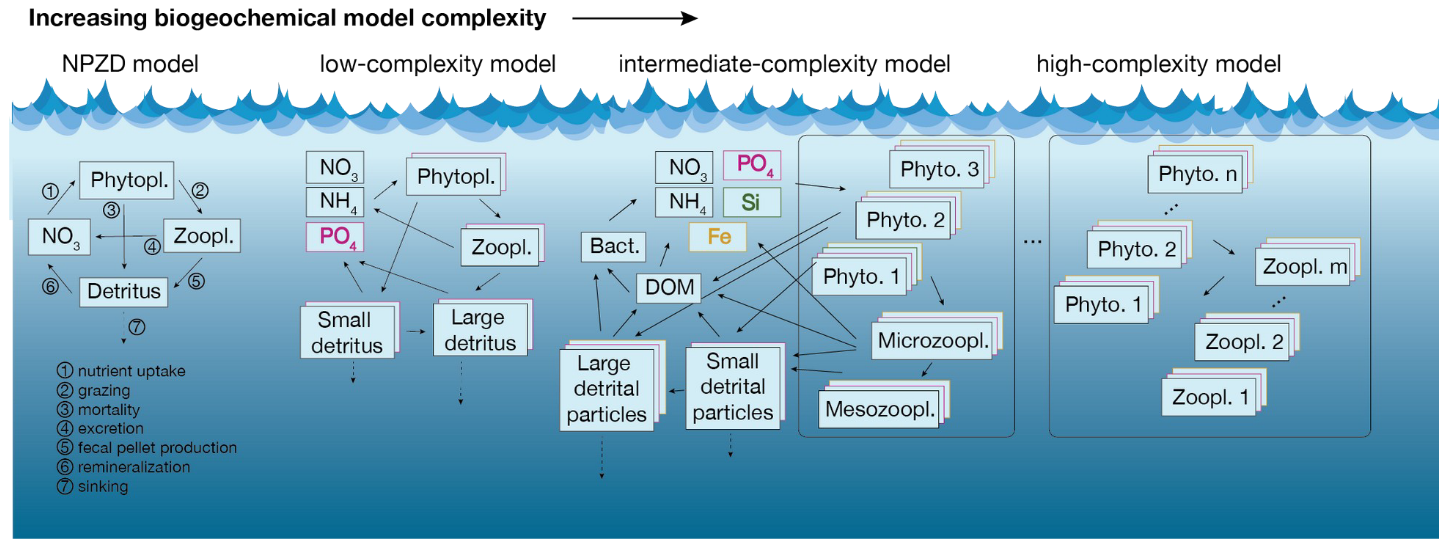
\includegraphics[width=1\linewidth]{figures/fennel22-bgc-complexity.png}
\end{figure}
\small{From \href{https://escholarship.org/uc/item/8219x0z0}{Fennel et al. (2022)}. Schematic representation of the state variables and biogeochemical transformations across a range of OBMs with increasing complexity from left to right. Squares represent state variables. Solid arrows represent selected transformations between state variables. Dashed arrows illustrate vertical sinking of particles.}
\end{frame}


%------------------------------------------------
\section{Elements of the Green Ocean models}
%------------------------------------------------
\begin{frame}{The green ocean: a quantitative description for biogeochemistry}
\begin{itemize}
\item In marine chemical--biological systems, problems are often more complex than in purely physical systems. The governing equations of the chemical--biological dynamics cannot be derived explicitly from conservation laws as in Newton's mechanics or in geophysical fluid dynamics.
\item The transport of biogeochemical constituents in the ocean must follow the rules of fluid dynamics, and therefore biogeochemical equations are coupled to physical equations in Ocean Biogeochemistry Models (OBM) or Green Ocean Models.
\item These equations must be derived from observations. Experimental findings can be translated into mathematical formulations that describe the process quantitatively. These functions represent the \textbf{response curves (or reaction norms)} and the interactions between drivers and state variables. The combination of these formulations constitutes a dynamical model.
\item \url{https://marine.copernicus.eu/explainers/operational-oceanography/monitoring-forecasting/models/green-ocean}
\end{itemize}
\end{frame}

%------------------------------------------------
\begin{frame}{Coupling Physics and BGC: Advection-Diffusion-Reaction Equations}
The conservation equations for tracers of an ocean model are extended with a reaction term, which is local (it does not directly depend on spatial gradients, but it can be affected by them in the overall solution). $R(C)$ is basically an ODE:
\[
\frac{\partial C}{\partial t}
+ \mathbf{u} \cdot \nabla C
= \nabla \cdot (K \nabla C) + R(C)
\]
This equation is now resolved at an increasingly high resolution: \url{https://www.gfdl.noaa.gov/visualization/visualizations-oceans/#}

In the vertical direction, this would look like
\[
\frac{\partial C}{\partial t}
= \frac{\partial}{\partial z}
\left(K_z \frac{\partial C}{\partial z}\right) + \dot{C}
\]
Notice that the biogeochemical rate of change $\dot{C}$ is the same in all three spatial directions.
\end{frame}

%------------------------------------------------
\begin{frame}{The Continuum Hypothesis in OBM}    
\begin{columns}
\column{0.3\linewidth}
\begin{figure}
    \centering
    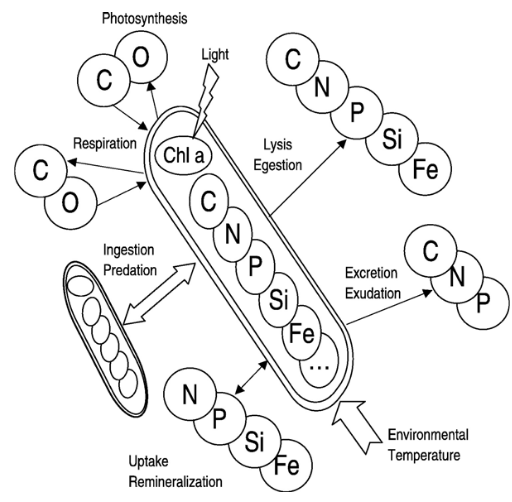
\includegraphics[width=1\linewidth]{figures/standard-organism-vichi.png}
    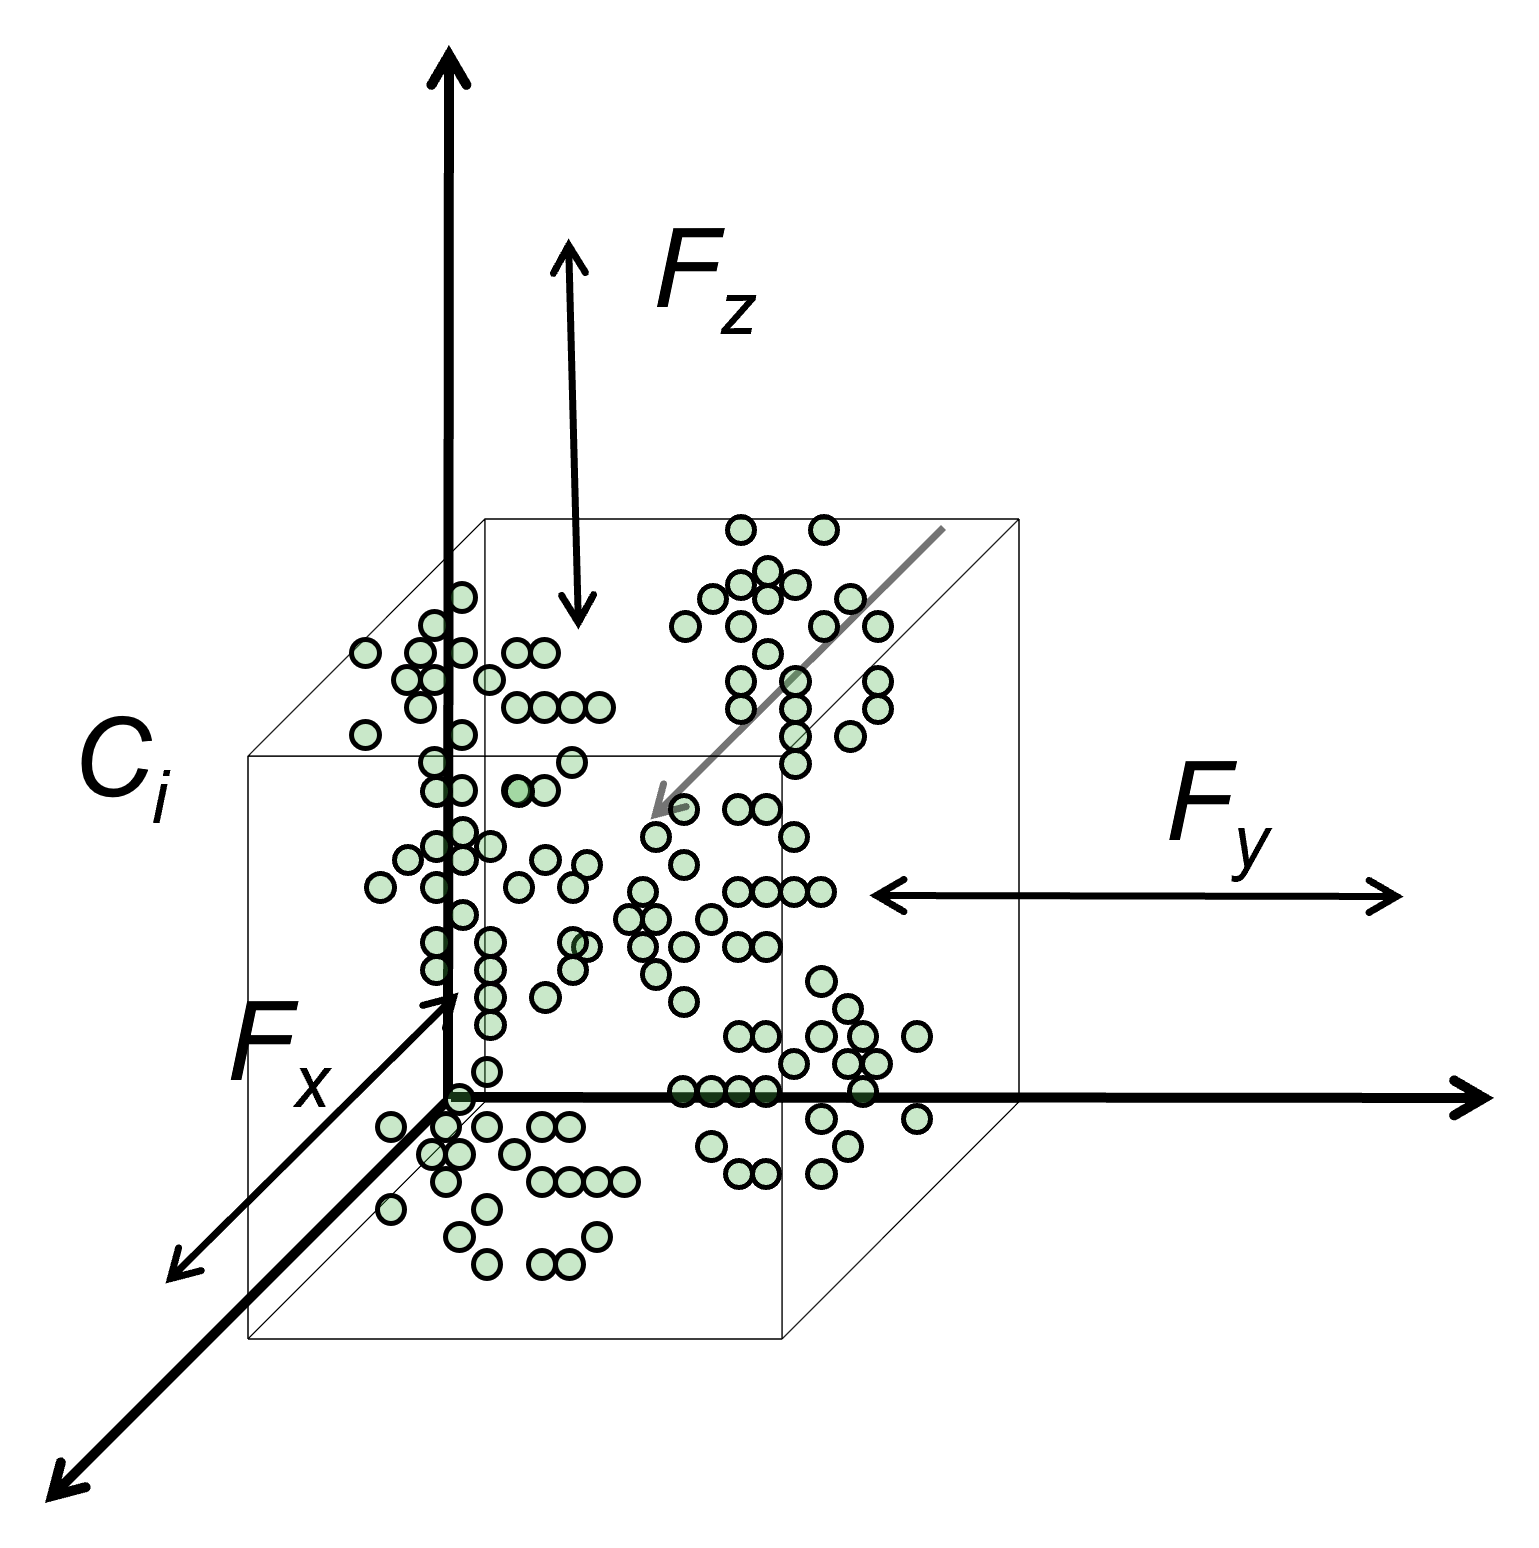
\includegraphics[width=0.8\linewidth]{figures/control_volume.png}
\end{figure}
\column{0.7\linewidth}
\vspace{-1cm}
\begin{figure}
    \centering
    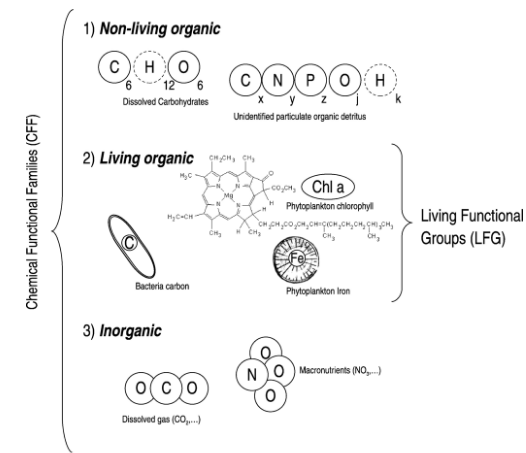
\includegraphics[width=0.6\linewidth]{figures/CFF-vichi.png}
\end{figure}
\vspace{-0.5cm}
\scriptsize{The field $C(\mathbf{x}, t)$ is a continuous function, such as temperature and salinity. In biomass-based OBMs it is assumed that the number of (equal) \textit{standard organisms} (like phytoplankton cells) is high and uniformly  distributed. They can thus be described by concentrations of \textit{virtual} chemical functional families (CFF, \href{https://doi.org/10.1016/j.jmarsys.2006.03.006}{Vichi et al., 2007}), which are continuous functions of space and time. The fluxes inside and around a control volume describe the processes that change the concentration of the CFF, which can have different currencies.}
\end{columns}
\end{frame}

%-------------------------------------------------
\begin{frame}{Optional Exercise US2.4-bgc01: Measuring Phytoplankton Biomass}
\begin{itemize}
\item {\small{}This exercise will show you the relevance of multiple currencies. Phytoplankton biomass can be measured in different ways and follows an exponential phase until resources become limiting or other factors control growth}{\small\par}
\item {\small{}The file }\texttt{\small{}data\textbackslash flynn94.csv}{\small{} contains data from a batch experiment conducted by Flynn et al. (1994). The full table and the related units are available in file }\texttt{\small{}flynn94.pdf}{\small{}.
}\emph{\small{}Flynn, K.J., Davidson, K., Leftley, J.W., 1994. Carbon-nitrogen relations at whole-cell and free-amino-acid levels during batch growth of Isochrysis galbana (Prymnesiophyceae) under conditions of alternating light and dark. Marine Biology 118, 229--237. https://doi.org/10.1007/BF00349789}{\small\par}
\item {\small{}Plot the data in a notebook and answer the following questions}{\small\par}
\begin{enumerate}
\item {\small{}Is the growth exponential? }{\small\par}
\item {\small{}Can you separate the growth curve into some phases?}{\small\par}
\item {\small{}How different is the growth expressed in cellular carbon from that measured in cell number and chlorophyll?}{\small\par}
\item {\small{}Is the ammonium consumption approximated by an exponential curve?}{\small\par}
\end{enumerate}
\end{itemize}
\end{frame}

%------------------------------------------------
\begin{frame}{A model of primary production in the ocean}
\scriptsize{This is the output of a numerical ocean--biogeochemistry model applied to simulate the observed \textbf{integrated primary production} at the Bermuda Atlantic Time Series (BATS). The comparison is done using monthly means (\href{https://bg.copernicus.org/articles/6/2333/2009/}{Vichi and Masina, 2009}). This output is the result of multiple interactive process models that generate an emergent behavior: the seasonal cycle of PP. \textit{Q: Why is integrated primary production a good state indicator? What are its drivers? At which temporal and spatial scales are they expected to change?}}
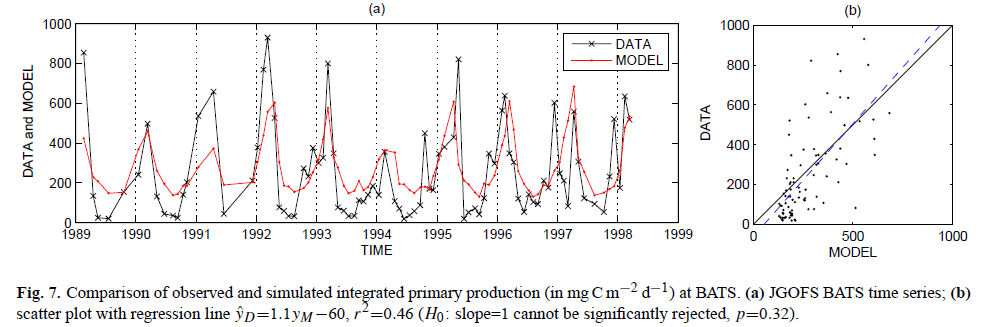
\includegraphics[width=0.9\paperwidth]{figures/PP_BATS}
\end{frame}


%------------------------------------------------
\begin{frame}{State variables, drivers and processes: which is which?}
\begin{itemize}
\item Nutrient uptake in phytoplankton is a function of concentration in surrounding water
\item Primary production in the ocean is a function of vertical mixing (light availability), temperature, and nutrient availability
\item Zooplankton predation is a function of available preys and search efficiency
\item Others?
\end{itemize}
\begin{alertblock}{Do they sound true but vague?}
A quantitative approach is necessary to define and express these relationships
\end{alertblock}
\end{frame}

%------------------------------------------------
\begin{frame}{Environmental drivers}
\begin{itemize}
    \item \textbf{A driver is a state variable}. It is used to drive component(s) of a system (i.e. other state variables) as an external condition, also known as one--way forcing. Environmental (or abiotic) drivers are identifiable physical features of the marine system, such as salinity, temperature, mixing, others?
    \item In the real marine system, there can be two-way forcings, feedback between state variables that affect the drivers (phytoplankton absorb light and changes the temperature of the ocean).   
\end{itemize} 
\end{frame}

%------------------------------------------------
\begin{frame}{Response curves (reaction norms)}
\begin{columns}
\column{0.5\linewidth}
\small{
\begin{itemize}
\item A \textbf{response curve} describes how certain species respond to one driver in laboratory settings
\item The physiological response can be expressed in terms of several indicator variables: photosynthetic rate, amount of oxygen consumed, specific growth rate, nutrient uptake, etc.
\item For instance, in the Southern Ocean, temperature is recognized to control the maximum growth rate of of diatoms. Other drivers may also affect the realized growth, such as nutrients and light.
\end{itemize}
}
\column{0.5\linewidth}
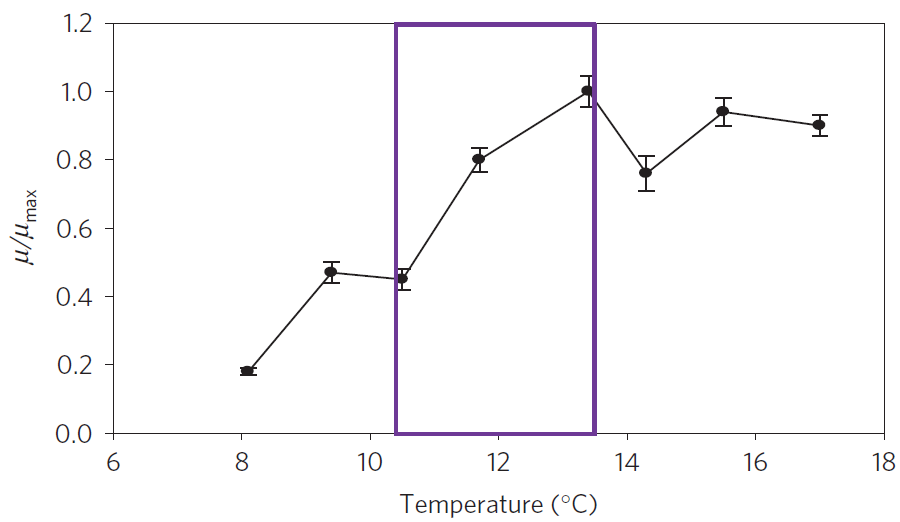
\includegraphics[scale=0.35]{figures/reaction_norm_T_boyd}
\scriptsize{A response curve of \emph{Prorocentrum multiseries} (\uline{\href{https://www.nature.com/articles/nclimate2811}{Boyd et al., 2016}}). Temperature bounds of the purple rectangle denote the mean (10.6$^{o}$C) for sub-Antarctic surface waters for present--day spring/summer and that projected (13.7$^{o}$C) for this province by 2100.
\textbf{Q: do we expect surface waters in the Southern Ocean to be constantly at this projected value?}}
\end{columns}
\end{frame}

%------------------------------------------------
\begin{frame}{Macroscopic response to temperature}
\footnotesize
\begin{columns}
\column{0.4\linewidth}
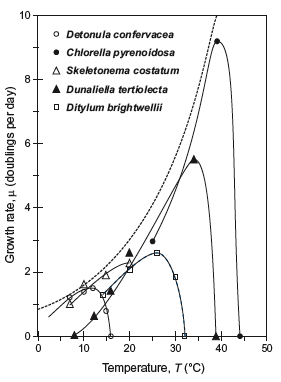
\includegraphics[width=5cm]{figures/eppley}
\column{0.6\linewidth}
\begin{itemize}
\item Physiological rates are controlled by environmental temperature.
\item (\href{https://spo.nmfs.noaa.gov/sites/default/files/pdf-content/1972/704/eppley.pdf}{Eppley, 1972}) demonstrated that single species are subject to temperature ranges, but taken as a population of algae in the ocean they are constrained by a curve envelope. He proposed the empirical equation
\[
\mu_{max}=0.59e^{0.0633T}
\]
\item The Eppley equation gives the maximum potential growth rate of the phytoplankton assemblage at each temperature. It is expressed in doubling per day (related to the number of cells).
\end{itemize}
\scriptsize
\textbf{Q: Is this a response curve?}
\end{columns}
\end{frame}

%------------------------------------------------
\begin{frame}{Functional response to light}
\scriptsize
\begin{columns}
\column{0.6\linewidth}
\begin{center}
\vspace{-0.7cm}
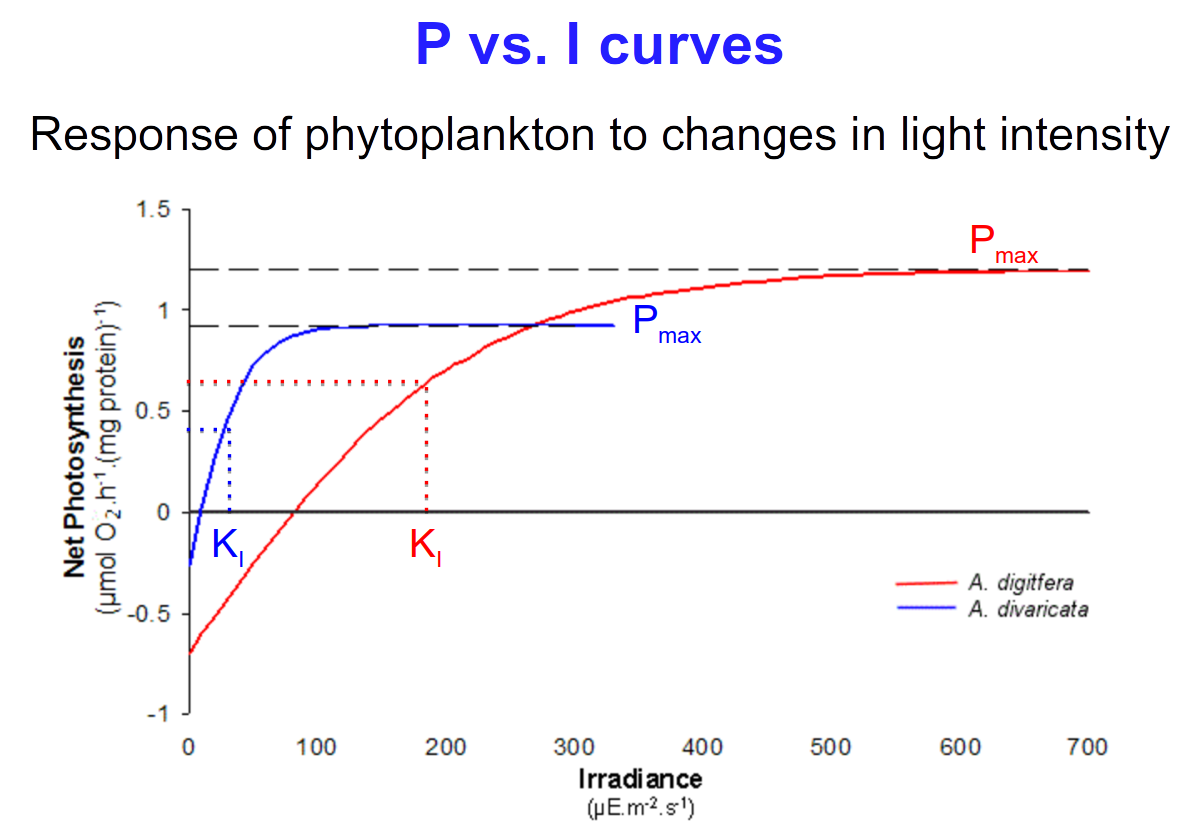
\includegraphics[width=5cm]{figures/P-I_Fawcett}
\vspace{-0.7cm}
\end{center}
\begin{itemize}
\item Several reaction norms have been proposed for phytoplankton response to light (\uline{\href{https://aslopubs.onlinelibrary.wiley.com/doi/10.4319/lo.1976.21.4.0540}{Jassby and Platt, 1976}})
\item The hyperbolic shape above follows eq (2)
\[
P\left(I\right)=P_{max}\alpha\frac{I}{\alpha I+P_{max}}
\]
where $\alpha$ is the linear slope of the curve in under--saturated light conditions and $I$ is the irradiance. \textbf{\emph{Q: Where is the half--saturation constant $K$ in this equation?}} \textbf{What are the units of $\alpha$?}
\end{itemize}
\column{0.4\linewidth}
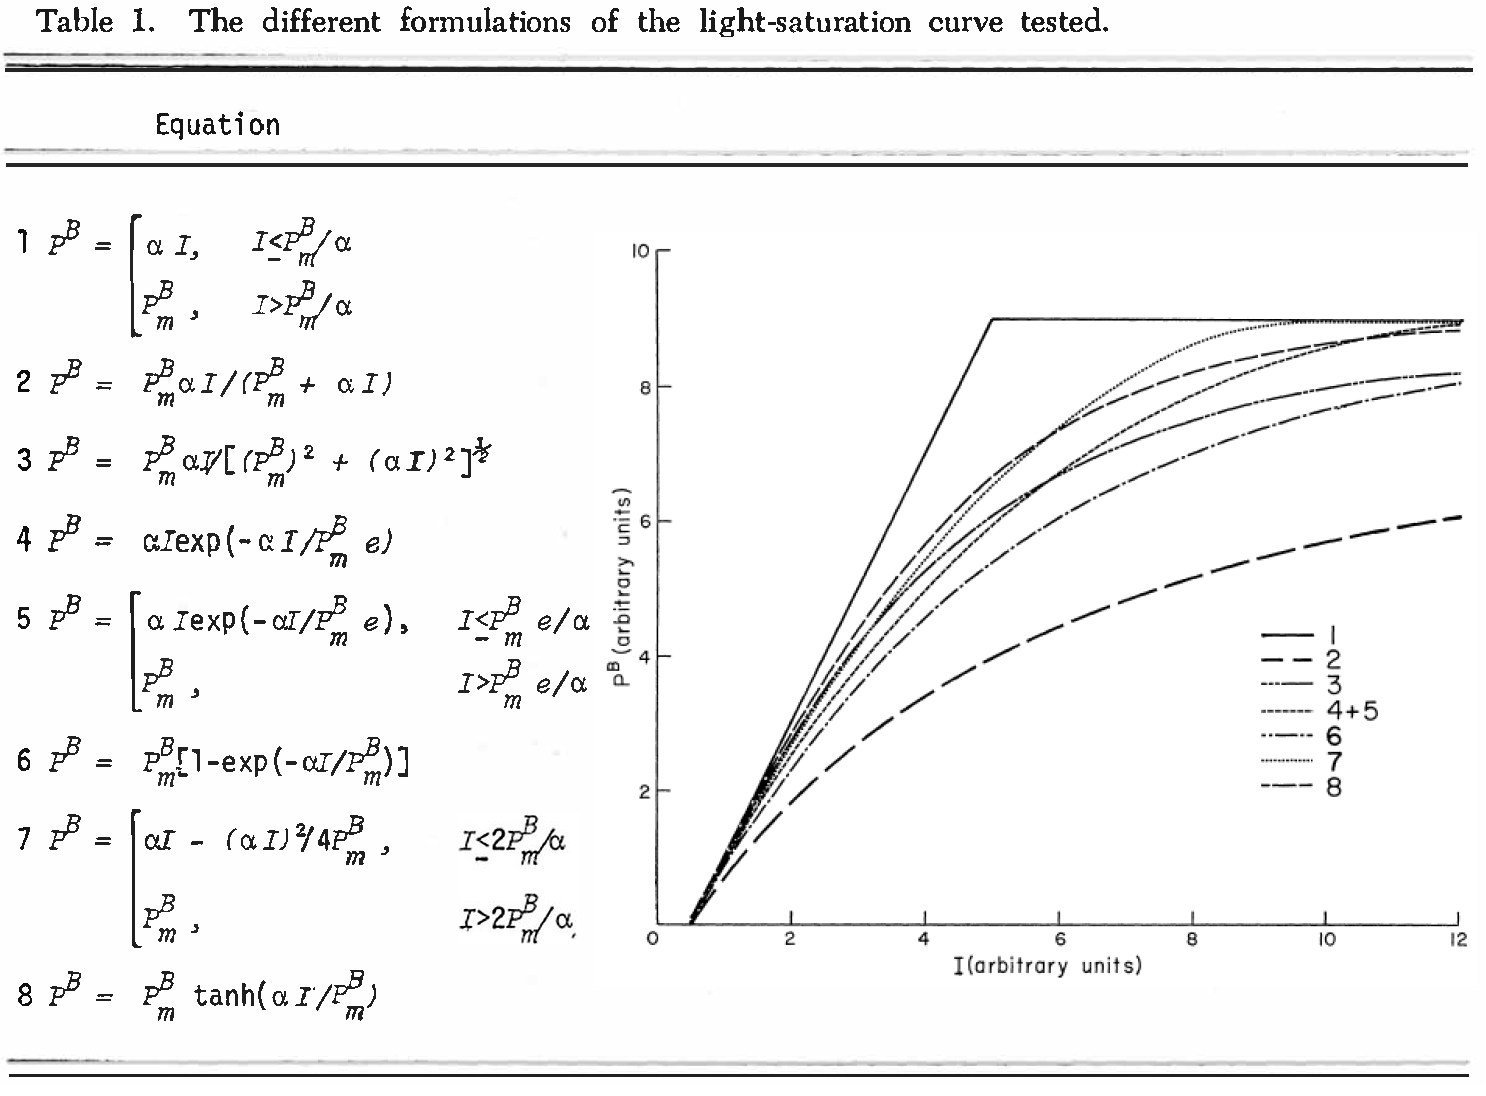
\includegraphics[width=1\linewidth]{figures/jassby_platt}
\end{columns}
\end{frame}

%------------------------------------------------
\begin{frame}{Functional response to nutrients}
\begin{columns}
\column{0.5\linewidth}
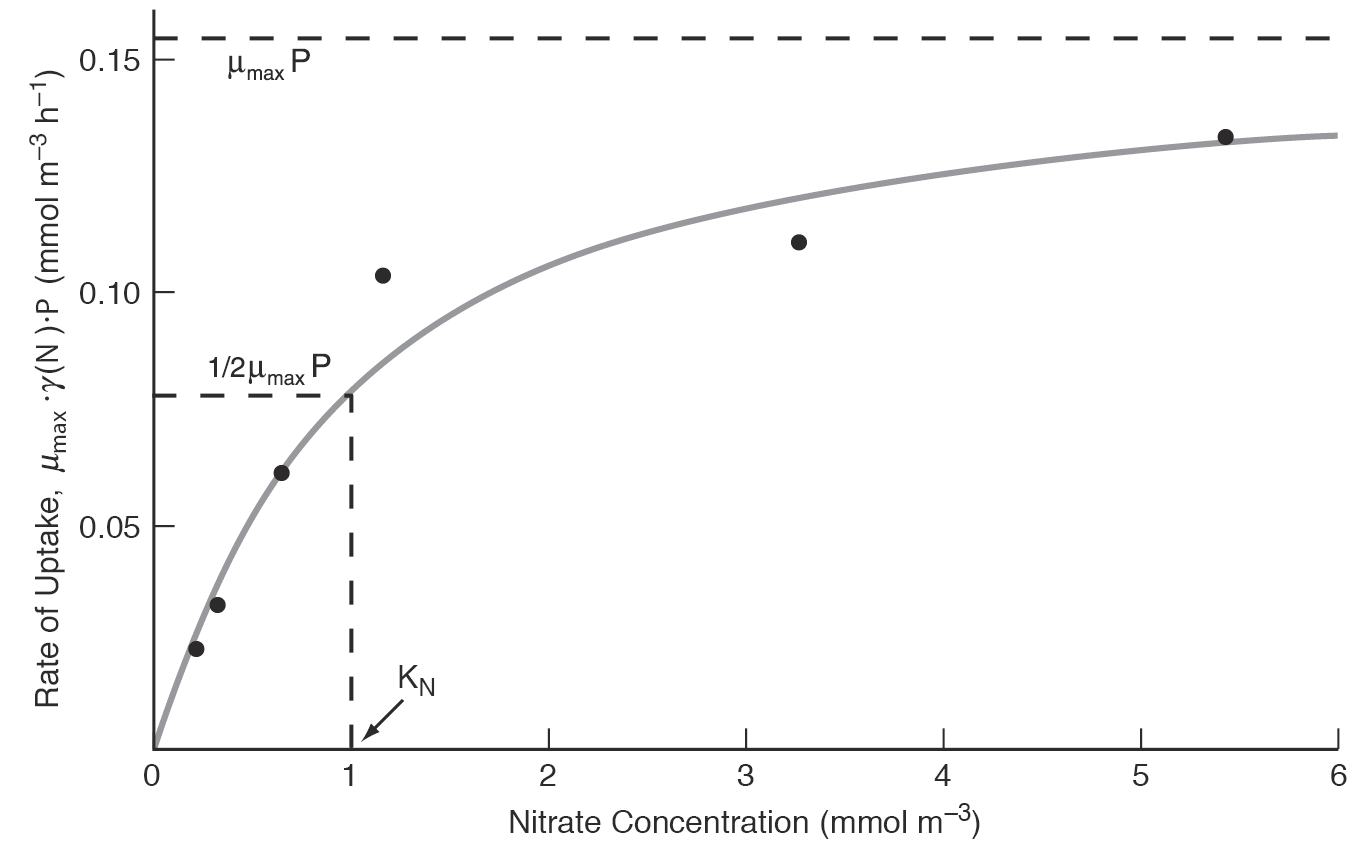
\includegraphics[width=7cm]{figures/MM}
\column{0.5\linewidth}
\small{
\begin{itemize}
\item The \textbf{rate of uptake} of dissolved nutrients from the water is a non-linear function of the environmental concentration. It's a function on one single variable $N$, the concentration of the nutrient (e.g. nitrate in mmol N m$^{-3}$)
\item Its functional form was proposed by \href{https://pubs.acs.org/doi/10.1021/bi201284u}{Michaelis and Menten (1913)} and \href{https://www.annualreviews.org/doi/10.1146/annurev.mi.03.100149.002103}{Monod (1949)}
\end{itemize}
\textbf{Q: What are the units of the parameters? Which part is unitless (non-dimensional)?}
\[
\mu\left(N\right)=\mu_{max}\frac{N}{N+K_{N}}
\]
}
\end{columns}
\end{frame}

\begin{frame}{Functional response to prey abundance}
\begin{columns}
\column{0.5\linewidth}
\small{In the '50s, Holling investigated how the predator's rate of prey's capture depended on the prey's abundance. He proposed three types, which have been later generalized to special cases of a full range of ecological functions \href{ https://doi.org/10.1890/0012-9623-95.3.200}{(Denny, 2014)}.
\begin{align*}
\text{Type I: } & f(R) = \alpha R \\
\text{Type II: } & f(R) = \frac{\alpha R}{1 + t\alpha R} \\
\text{Type III: } & f(R) = \frac{aR^2}{1 + t\alpha R^2} \\
\text{General: } & f(R) = \frac{aR^n}{1 + t\alpha R^n}
\end{align*}}
\column{0.5\linewidth}
\begin{figure}
    \centering
    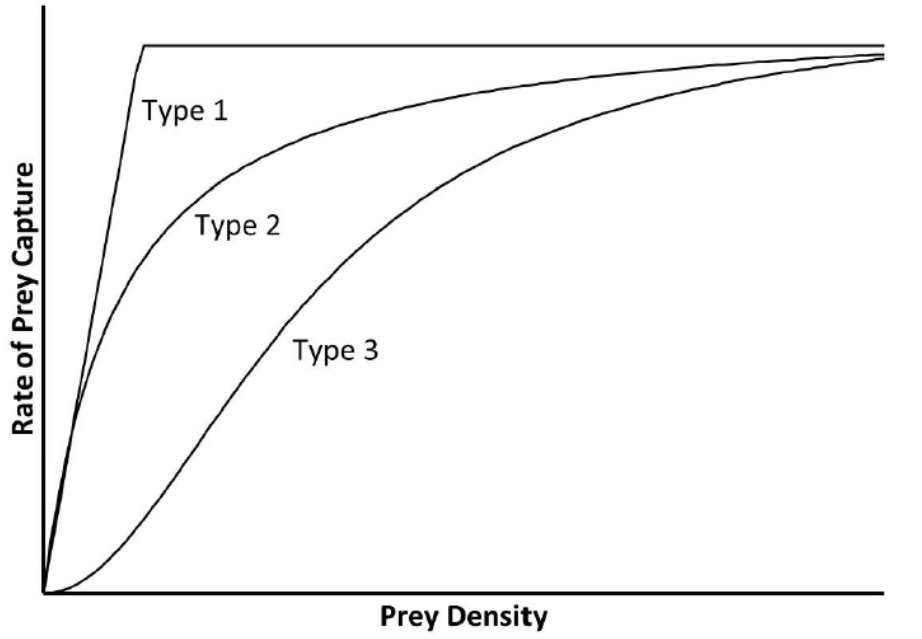
\includegraphics[width=1\linewidth]{figures/holling.png}
\end{figure}
\end{columns}
\end{frame}

%------------------------------------------------
\begin{frame}{Parameterization of a response curve}
\footnotesize
\begin{columns}
\column{0.5\linewidth}
\begin{itemize}
\item Organic carbon in the ocean is remineralized through respiration. Also, phytoplankton respiration depends on temperature. Lassiter (1975) proposed a \textbf{non-linear function}
\item This continuous mathematical function is asymmetrical with domain $\left]-\infty,+\infty\right[$; the curve is defined by 2 major parameters: the optimal and maximum temperatures
\[
f(x)=\begin{cases}
R_{0}e^{A\left(x-T_{opt}\right)}\left(\frac{T_{max}-x}{T_{max}-T_{opt}}\right)^{A\left(T_{max}-T_{opt}\right)} & x<T_{max}\\
0 & x\geq T_{max}
\end{cases}
\]
\end{itemize}
\column{0.5\linewidth}
\includegraphics[width=1\linewidth]{figures/respiration}
\end{columns}
\end{frame}


%-------------------------------------------------
\section{Simple dynamical models based on ODE}
%-------------------------------------------------
\begin{frame}{Malthusian growth model}
\begin{itemize}
\item All biogeochemical processes involve growth, and its first description was made by Malthus in the 18th century.
\item The derivation of the Malthusian model is based on the concept that growth rate is proportional to the population abundance. The independent variable is time, and there is an increase in the population with time that is expressed as 
\[
\Delta N=\mu N\Delta t
\]
where the growth rate $\mu$ is in units of 1/time.
\item We put this equation in differential form and obtain what is called
the dynamics of the exponential growth model 
\begin{equation}
\frac{dN}{dt}=\mu N\label{eq:malthus}
\end{equation}
\end{itemize}
\end{frame}

%-------------------------------------------------
\begin{frame}{Light attenuation: the Lambert-beer equation}
\begin{columns}
\column{8cm}
\begin{itemize}
\item \small{Life in the ocean comes from primary production, which depends on light availability.}
\item {\small{}Light is attenuated of a certain fraction along its pathway through the water, which is characterized by an attenuation coefficient $\varepsilon$ (units are 1/length)}
\item 
\[
I_{1}=I_{0}-\varepsilon I_{0}\ell\Rightarrow\Delta I=-\varepsilon I\Delta z
\]
\end{itemize}
\column{4cm}
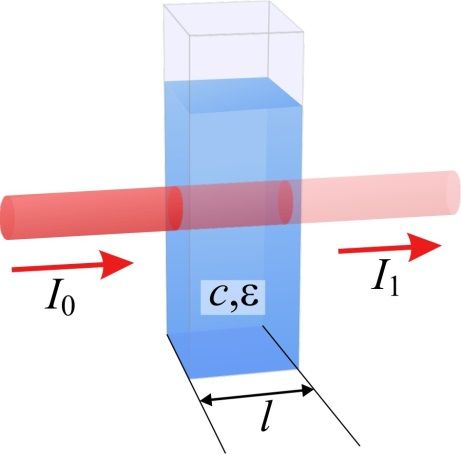
\includegraphics[scale=0.6]{figures/lambert-beer}
\end{columns}
\begin{itemize}
\item By putting it in differential form, one obtains the Lambert-Beer equation
\begin{equation}
\frac{dI}{dz}=-\varepsilon I\label{eq:decay}
\end{equation}
which can be solved analytically with the boundary condition $I(z=0)=I_{0}$
\[
I(z)=I_{0}e^{-\varepsilon z}
\]
\end{itemize}
\end{frame}

%-------------------------------------------------
\begin{frame}{Biogeochemical/ecological models that can be described with ODEs}
\begin{definition}
A system of (coupled) ODEs is a combination of ODE equations where the state variables interact with each other. 
\end{definition}
This is an initial value problem. We know the initial state of the system and want to determine the time evolution of the state variables
\begin{itemize}
\item {\small{}A (biogeo)chemical system with multiple reactions ($A+B\Rightarrow C+D$) }{\small\par}
\item {\small{}A system with prey-predator interactions (a trophic web, like primary producers and grazers)}{\small\par}
\item {\small{}A physiological model describing biochemical transformations (carbon biomass formation through photosynthesis driven by light availability)}{\small\par}
\end{itemize}
These models are usually called \textbf{box models}: they are characterized by the dynamical co-existence of the state variables in the same enclosure.
\textbf{Very important:} exchanges with the region(s) outside the
system are known or negligible 
\end{frame}

%-------------------------------------------------
\begin{frame}{Initial value problems in biology/biogeochemistry}
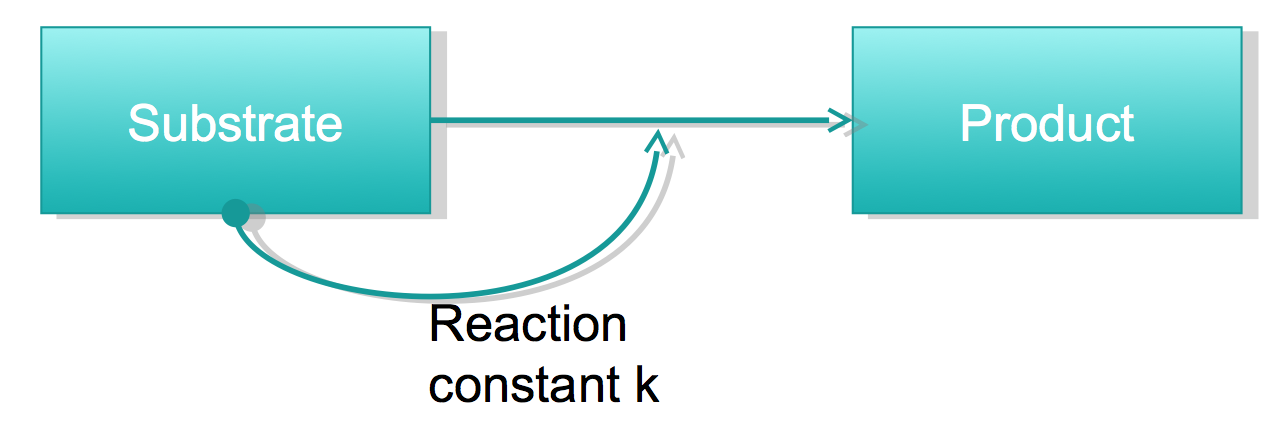
\includegraphics[scale=0.3]{figures/substrate}
{\scriptsize{}A simple chemical reaction model where the substrate is transformed into a product: $\mathrm{substrate\stackrel{k}{\Longrightarrow}}\mathrm{product}$}{\scriptsize\par}

{\scriptsize{}It is based on the concept that the }\textbf{\scriptsize{}transformation
rate is proportional to the chemical equilibrium constant and to the concentration of the substrate}{\scriptsize{}. The equations are a direct consequence of the mass conservation principle: the rate of change of the substrate is equal and opposite to the rate of change of the product:
\begin{equation}
\frac{dS}{dt}+\frac{dP}{dt}=\frac{d\left(S+P\right)}{dt}=0\label{eq:mass_conservation}
\end{equation}
}{\scriptsize\par}

{\scriptsize{}It is described by a system of 2 variables $S(t)$,
$P(t)$ and 2 ODEs
\begin{align*}
\frac{dS}{dt}= & -kS\\
\frac{dP}{dt}= & kS
\end{align*}
where the first one is the decay equation and the second one is Malthusian growth. Any initial value problem needs }\textbf{\scriptsize{}initial
conditions}{\scriptsize{}, $S(t=0)=S_{0}$, $P(t=0)=P_{0}$}{\scriptsize\par}
\end{frame}

%-------------------------------------------------
\begin{frame}{Analytical solutions}

Some ODEs like the decay or Malthusian growth can be integrated by separation of variables (see the Malthusian equation \ref{eq:malthus});
other ODEs can be solved by substitution of variables, or trigonometric equations. All the ODEs that can be analytically solved are tabulated (best reference: CRC Standard Mathematical Tables, Zwillinger, 2002). 

The first equation is solved and then the solution goes into the second equation which is again solved by separation of variables with the application of the initial conditions. In this specific case, it is easier to use eq. (\ref{eq:mass_conservation}) $P+S=P_{0}+S_{0}$,
which is valid for every $t$ $\left(\forall t\right)$ to derive
the solution
\begin{align*}
S(t)= & S_{0}e^{-kt}\\
P(t)= & P_{0}+S_{0}-S_{0}e^{-kt}
\end{align*}
Note that the substrate will never be exactly 0.
\end{frame}

\begin{frame}{Resource and consumer}

\includegraphics[scale=0.4]{figures/resource-consumer}
{\scriptsize{}Let's analyse a system with one resource and one consumer (e.g. phytoplankton and one dissolved nutrient like ammonium). If we assume that the rate of change of the resource is }\textbf{\scriptsize{}only controlled by the consumer}{\scriptsize{} (as in the previous case) according to the uptake rate and the abundance we write: 
\[
\frac{dN}{dt}=-kP
\]
But then the application of mass conservation gives 
\[
\frac{d\left(P+N\right)}{dt}=0\longrightarrow\frac{dP}{dt}=kP
\]
which is the infinite Malthusian growth that by definition is not
resource-limited. }\textbf{\scriptsize{}This set of ODE does not work to model this system}{\scriptsize{} because the}\textbf{\scriptsize{} resource should also control the consumption rate}{\scriptsize{} (see the different shape of the arrow in the graph, which means dependence,
as opposed to a normal arrow that indicates direct relationship)}{\scriptsize\par}
\end{frame}

%-------------------------------------------------
\begin{frame}{Limits to growth}
\begin{columns}
\column{0.5\linewidth}
\begin{itemize}
\item {\small{}Growth with limited resources is by definition a non-linear model and we need to adjust the functional form of the equation and include a new parameters that has not only units \textit{over time} but also \textit{over concentration} }
\end{itemize}
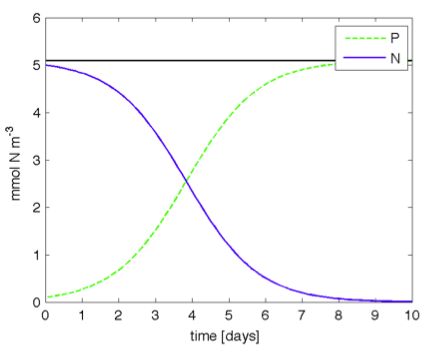
\includegraphics[width=0.8\linewidth]{figures/limits-growth-NP}
\column{0.5\linewidth}
\vspace{-1cm}
{\small{}
\begin{align}
k= & k'N\nonumber \\
\frac{dN}{dt}= & -k'NP\label{eq:limited_growth}\\
\frac{dP}{dt}= & k'NP\nonumber 
\end{align}
}{\small\par}
\begin{itemize}
\item {\small{}In this case, the growth of the consumer is limited by the resource. This system has the analytical solution
\begin{align*}
P+N= & P_{0}+N_{0}\\
P(t)= & P_{0}\frac{P_{0}+N_{0}}{P_{0}+N_{0}e^{-k'\left(P_{0}+N_{0}\right)t}}
\end{align*}
}{\small\par}
\end{itemize}
\end{columns}

\end{frame}

\begin{frame}{Numerical time integration: ODE solvers}
\begin{itemize}
\item Most natural systems can only be described with mathematical models that do not have an analytical solution
\item But we do not need to do the full derivation and write the computer code for each case.
\item There exist several numerical methods based on \textbf{finite differences} and they are grouped under the name of \textbf{ODE solvers}. In the next tutorial and in the exercise on the LV model, we will use the python ODE solver called \texttt{odeint} from the \texttt{scipy} module.
\item They basically require you to input the right hand side of the differential equations and then use it to compute the solution forward in time at discrete time intervals.
\end{itemize}
\end{frame}
%-------------------------------------------------
\begin{frame}{Tutorial: Limited Growth}
\begin{itemize}
\item We will write python code to plot the analytical solution of the NP model above to study the time evolution of phytoplankton and nutrient concentrations and analyse its dependency on the parameter and initial conditions.
\item We will then write the equations for a new model simulating the nutrient-phytoplankton-detritus system (NPD). We will include a detritus variable D that is produced from the mortality of phytoplankton and it is remineralized as a nutrient. We will need 2 additional parameters: the mortality rate (phytoplankton lysis) and the remineralization rate.
\end{itemize}
\end{frame}

%-------------------------------------------------
\begin{frame}{More complex models}
\begin{itemize}
\item Model building is a delicate process, which takes different nuances depending on the group of people doing it and the specific discipline
\item There is no \emph{one-size-fits-all} or universal recipe for building a model that describes a certain aspect of the marine environment
\item A useful introduction is given by Glover et al. (2011) in their Chapter 9 (available in the document folder). We will use their example 9.3 to explore the prey-predator interactions with the Lotka-Volterra model 
\end{itemize}
\end{frame}

%-------------------------------------------------
\begin{frame}{The Lotka-Volterra model}
\begin{itemize}
\item {\footnotesize{}Volterra (1926) wanted to study prey-predator interactions in fish population; Lotka (1920;1925) studied chemical oscillations between reagents and products}{\footnotesize\par}
\item {\footnotesize{}The model describes the interaction between two populations. The prey $X_{1}$ grows following the Malthusian equation and is consumed by the predator $X_{2}$ similarly to the resource-consumer model. The latter dies according to a constant decay term:
\begin{align*}
\frac{dX_{1}}{dt} & =X_{1}\left(p_{1}-p_{2}X_{2}\right)\\
\frac{dX_{2}}{dt} & =X_{2}\left(p_{2}p_{3}X_{1}-p_{4}\right)
\end{align*}
}{\footnotesize\par}
\item {\footnotesize{}The presence of the parameter $p_{3}$ implies that there is no mass conservation, because the predator is not efficient in translating the ingestion rate into growth. Some mass from the prey is lost to the environment}{\footnotesize\par}
\item \textbf{\footnotesize{}Please note that this not a realistic model: it has major assumptions}{\footnotesize{} (}{\footnotesize{}\uline{read
more about them in the textbook chapter}}{\footnotesize{}): 1) The prey population is not resource limited. 2) The food supply of the predator population depends entirely on the prey populations. 3) The predator mortality is proportional to the population size. 4) The environment does not change as well as the type of preys and predators.}{\footnotesize\par}
\end{itemize}
\end{frame}

%-------------------------------------------------
\begin{frame}{Model description (from Glover et al 2011)}

\begin{center}
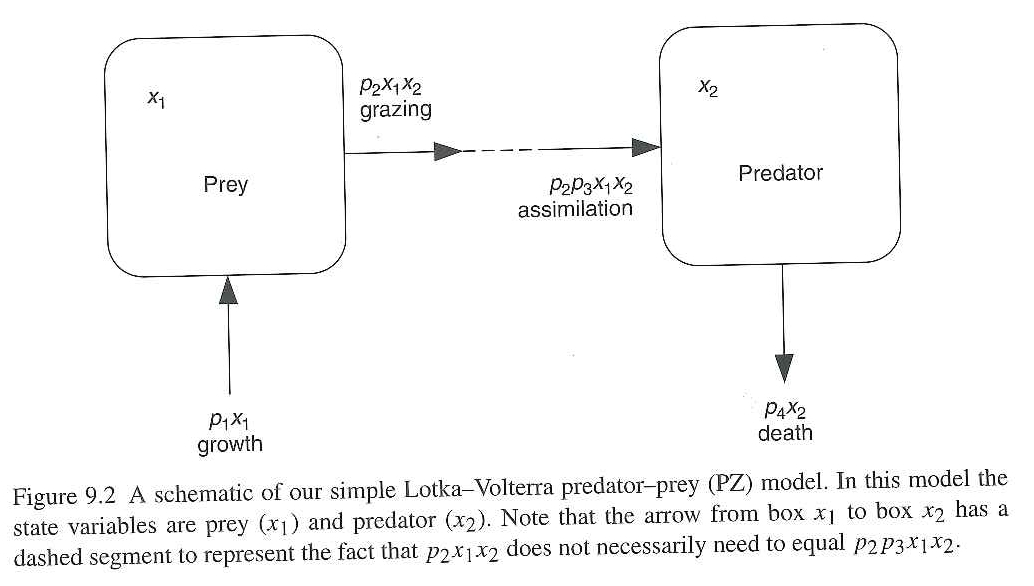
\includegraphics[scale=0.8]{figures/LV-scheme}
\par\end{center}

\end{frame}

%-------------------------------------------------
\begin{frame}{A numerical solution from Glover et al (2011)}

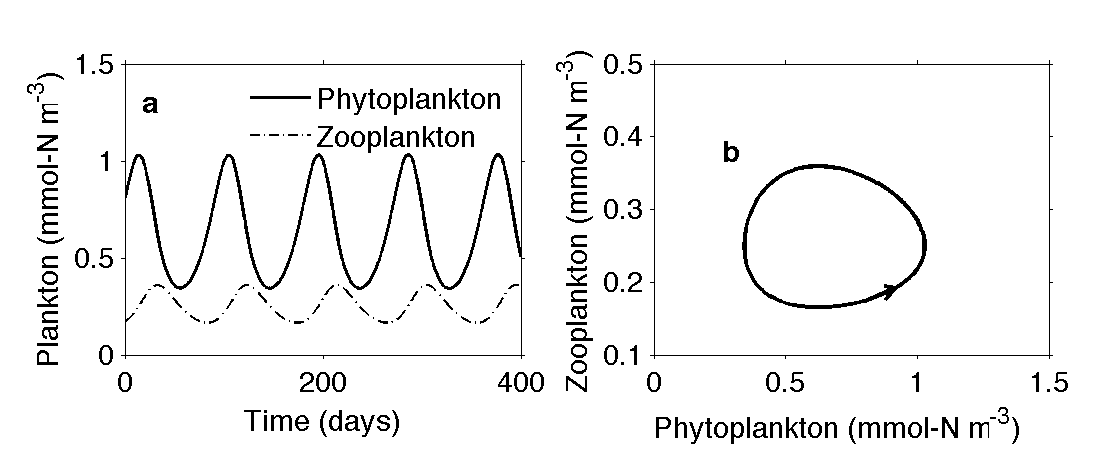
\includegraphics[scale=0.5]{figures/ftut_LVpzts1}
The LV model is nowadays used mostly for educational purposes, because it allows a rigorous analysis to illustrate the major aspects of mathematical biology and it is a tractable example of numerical solution of ODE systems. Moreover, it does contain elements that are common to any marine model.
\end{frame}

%-------------------------------------------------
\begin{frame}{Exercise US2.4-bgc02: Lotka-Volterra model}
\begin{itemize}
\item {\small{}The L-V model cannot be solved analytically. The code is available in the python notebook}\texttt{\small{} LV\_pz.ipynb}{\small{}. Run the code to reproduce the panel a from the previous figure}
\item {\small{}Modify the notebook to answer the following questions and submit the PDF on Amathuba.}
\begin{enumerate}
\item {\small{}Write the code to plot panel b (the phase space) in the appropriate cell block}
\item {\small{}Set the parameter $p_{3}=1$ and compare how different the trajectory is in the phase space}
\end{enumerate}
\end{itemize}
\end{frame}

%------------------------------------------------
\section{It's a wrap...}
%------------------------------------------------
\begin{frame}{What is Biogeochemical Modelling? (Core Concepts I)}
\begin{itemize}
    \item \textbf{Integration of disciplines:} Combines physics, chemistry, and biology to describe ocean ecosystems
    \item \textbf{Mass balance framework:} All models track stocks and flows via  
    \[
    \frac{dC}{dt} = \text{sources} - \text{sinks}
    \]
    \item \textbf{Empirical biology:} Unlike physics, biological processes are parameterized from observations (response curves, assumptions)
    \item \textbf{State variables \& trophic structure:} Ecosystems represented as compartments (e.g. nutrients, phytoplankton, zooplankton) linked by fluxes
\end{itemize}
\end{frame}

%-----------------------------------
\begin{frame}{What is Biogeochemical Modelling? (Core Concepts II)}
\begin{itemize}
    \item \textbf{Drivers vs processes:}
    \begin{itemize}
        \item Drivers = environmental controls (light, temperature, nutrients)
        \item Processes = growth, uptake, predation described by nonlinear response functions
    \end{itemize}
    \item \textbf{Coupled system:} Ocean BGC models link biology to circulation via advection--diffusion--reaction equations
\end{itemize}
\textbf{Key message:} Biogeochemical models are data--driven, coupled dynamical systems representing ecosystem interactions and environmental forcing.
\end{frame}

%-----------------------------------
\begin{frame}{How We Model Ocean Biogeochemistry (Approaches)}
\begin{itemize}
    \item \textbf{Model hierarchy (increasing complexity):}
    \begin{itemize}
        \item Simple: NP, NPZD box models (ODEs)
        \item Intermediate: Fasham--type (multi--compartment)
        \item Advanced: Green Ocean models (fully coupled systems)
    \end{itemize}
    \item \textbf{Mathematical backbone:}
    \begin{itemize}
        \item ODE systems for local ecosystem dynamics (box models)
        \item Reaction terms represent biological rates
        \item Often require numerical solvers (no analytical solution)
    \end{itemize}
\end{itemize}

\end{frame}
%-----------------------------------
\begin{frame}{How We Model Ocean Biogeochemistry (Insights)}
\begin{itemize}
    \item \textbf{Key ecological principles:}
    \begin{itemize}
        \item Growth is often exponential, but resource--limited (nonlinear)
        \item Ecosystem interactions (e.g. predator--prey) generate complex dynamics
        \item Environmental forcing (especially energy, turbulence, light) strongly shapes biogeochemical dynamics
    \end{itemize}
    \item \textbf{Critical modelling choices:}
    \begin{itemize}
        \item Selection of state variables \& currencies (C, N, biomass, etc.)
        \item Choice of functional responses (e.g. Michaelis--Menten, light curves, temperature response)
        \item Trade-off between complexity vs interpretability
    \end{itemize}
\end{itemize}
\textbf{Key message:} Ocean biogeochemistry models range from simple conceptual ODE systems to complex coupled simulations, but all rely on nonlinear interactions, environmental forcing, and careful parameterization.
\end{frame}

\end{document}